%\PassOptionsToPackage{backref}{hyperref}
%  JRFM (Journal of Risk and Financial Management) - MDPI Format
%  Validating LLM Structural Reasoning: Detecting Persistent Market Regimes
%  Through Temporal Obfuscation
%
\documentclass[jrfm,article,accept,moreauthors,pdftex]{Definitions/mdpi}

\firstpage{1}
\makeatletter
\setcounter{page}{\@firstpage}
\makeatother
\pubvolume{1}
\issuenum{1}
\articlenumber{0}
\pubyear{2026}
\copyrightyear{2026}
\externaleditor{ } % More than 1 editor, please add `` and '' before the last editor name
\datereceived{29 March 2026}
\daterevised{2 May 2026} % Comment out if no revised date
\dateaccepted{14 May 2026}
\datepublished{ }

%% Additional packages
\usepackage{placeins}  % for \FloatBarrier
%
%%% Commands not defined in this version of mdpi.cls
%\newcommand{\dataavailability}[1]{%
%\vspace{6pt}\noindent{\fontsize{9}{9}\selectfont\textbf{Data Availability Statement:} {#1}\par}}
%\newcommand{\disclaimer}[1]{%
%\vspace{6pt}\noindent{\fontsize{9}{9}\selectfont\textbf{Disclaimer/AI Statement:} {#1}\par}}
%\newcommand{\institutionalreview}[1]{%
%\vspace{6pt}\noindent{\fontsize{9}{9}\selectfont\textbf{Institutional Review Board Statement:} {#1}\par}}
%\newcommand{\informedconsent}[1]{%
%\vspace{6pt}\noindent{\fontsize{9}{9}\selectfont\textbf{Informed Consent Statement:} {#1}\par}}


%=================================================================
\Title{Temporal Obfuscation Testing for LLM Structural Reasoning: From Single-Day Dealer Constraints to Persistent Market Regimes}

% Author ORCID IDs
\newcommand{\orcidauthorA}{0009-0009-3777-6148}
\newcommand{\orcidauthorB}{0000-0002-8661-8877}

% Authors
\Author{\hl{Christopher Regan} %MDPI: 1. Please carefully check the accuracy of names and affiliations. 2. This name is different from the one submitted online at susy.mdpi.com. Please confirm which is correct.
 *\orcidA{} and \hl{Ying Xie} %MDPI: Please check and confirm whether this is the corresponding author, since this information is not consistent with that submitted online at susy.mdpi.com.
 \orcidB{}}
 %MDPI: Dear Authors,
%(1) Please proofread the article format according to the comments left and pay attention to the highlighted parts.
%(2) Please do not delete the comments and do not remove highlight during your proofreading, since we need to check point by point after receiving your proofed version.
%(3) Please just modify or confirm or give feedback.
%(4) English editing and layout have been complete, please do not revert the changes.
%(5) Changing authorship is NOT acceptable during this period (including adding new authors/corresponding authors/affiliations or deleting present authors/corresponding authors/affiliations or exchanging author orders).

% Authors for PDF metadata
\AuthorNames{Christopher Regan and Ying Xie}

% Affiliations
\address[1]{%
 College of Computing and Software Engineering, Kennesaw State University, Marietta, GA 30060, USA; \hl{yxie2@kennesaw.edu} %MDPI: We added this email address here according to that submitted online at susy.mdpi.com. Please confirm.
}

% Corresponding author
\corres{\hangafter=1 \hangindent=1.05em \hspace{-0.82em} Correspondence: cregan1@kennesaw.edu}

% Abstract — IMRAD structure without headings, per MDPI guidelines
\abstract{Deploying large language models (LLMs) for domain-specific analysis raises a critical validation challenge: distinguishing genuine structural reasoning from training data memorization. We address this through temporal obfuscation testing, which strips calendar dates, ticker symbols, and contextual markers from input sequences, forcing models to reason from numerical structure alone. Applying this framework to options dealer gamma exposure (GEX) patterns across two temporal scales, we validate detection using \highlighting{2221}~evaluations %MDPI: Commas are only used for numbers with five or more digits. We have removed them in four-digit numbers. Please review and confirm throughout the manuscript.
 (1412 real windows plus 809 synthetic controls) spanning 2020--2025. At the single-day scale, obfuscation testing achieves 71.5\% detection of dealer hedging patterns with 91.2\% predictive accuracy; raw strike-level data outperforms pre-calculated GEX metrics by \mbox{30.8 percentage} points (92.3\% vs.\ 61.5\%), establishing that parametric aggregation represents lossy compression of structural signal. At the multi-day scale, 30-day regime detection achieves 81.2\% detection in 2024 (95\% CI [75.8, 86.1]\%) versus 12.1\% in 2020 (95\% CI \mbox{[8.1, 16.6]\%})---a 69.1 percentage point separation ($\varphi = 0.69$, Fisher's exact $p = 1.8 \times 10^{-52}$)---with 0\% false positives on synthetic controls. Multi-year analysis reveals regime evolution tracking zero-days-to-expiration (0DTE) adoption---detection rising from 3.7\% (2021) to 100\% (2024)---with GEX magnitude growing from \$3.0B to \$20.3B. Stable detection despite collapsing profitability (Sharpe 1.8 $\rightarrow$ 0.1) confirms structural market mechanics rather than exploitable inefficiencies, establishing temporal obfuscation as a generalizable methodology for validating LLM reasoning in quantitative domains.}

% Keywords (semicolon-separated per MDPI style)
\keyword{LLM validation; structural reasoning; temporal obfuscation; regime detection; market microstructure; gamma exposure; zero-days-to-expiration options; options \mbox{market structure}}

%=================================================================
\begin{document}

\section{Introduction}
\label{sec:introduction}

Deploying large language models (LLMs) for domain-specific quantitative analysis raises a first-order validation problem: distinguishing outputs produced by genuine structural reasoning about the domain from outputs produced by surface-level pattern recall of training-corpus text \citep{mccoy2023embers}. The problem is especially acute in finance, where news and analyst coverage of well-known events (the 2020 COVID crash, the 2021 meme-stock episode, the 2023 banking stress) are heavily represented in training data, and where the most structurally interesting patterns occurred in years the model has seen.

This paper proposes \textbf{\hl{temporal obfuscation testing}} %MDPI: Please confirm if the bold formatting is necessary; if not, please remove it. Please review and confirm throughout the manuscript.
as a validation methodology for this problem and applies it to options dealer gamma-exposure (GEX) regimes. The method strips calendar dates, ticker symbols, and any contextual identifiers from input sequences and re-evaluates an LLM on the stripped input. When obfuscated detection rates remain high and discriminate persistent regimes from synthetic controls, the model's performance cannot be attributed to memorization of the underlying dates; when they collapse, memorization is the parsimonious explanation. We use dealer GEX as the demonstration domain, because it combines mechanically grounded constraints (dealers \emph{\hl{must}} %MDPI: Please confirm if the italics are necessary; if not, please remove them. Please review and confirm throughout the manuscript.
hedge delta under regulatory and risk-management rules) with a sharp natural contrast---2020 (pre-0DTE, episodic dealer positioning) versus 2024 (post-0DTE, sustained structural dealer positioning)---that a genuinely reasoning system should separate on structural grounds alone \citep{ni2005stock,garleanu2009demand,dim2023odtes}.

\paragraph{\hl{Research gap.}}%MDPI: Please confirm if it should be formatted as list or as title.
Prior work has, independently, (i)~characterized dealer-gamma hedging and its microstructure effects (\citealp{ni2005stock,garleanu2009demand,anderegg2022impact,dim2023odtes,adams2025zerodte}; among others); (ii)~documented the rapid growth of zero-days-to-expiration (0DTE) options between 2022 and 2025 and its implications for intraday volatility \citep{cboe2024zero,cboe2025spx0dte,fishman2023gamma}; and (iii)~evaluated LLM reasoning with probing and chain-of-thought techniques in non-financial domains \citep{wei2022chain,kojima2022large,mccoy2023embers}. What is missing is a method for validating LLM structural reasoning \emph{within} financial microstructure that (a)~controls for training-data memorisation of specific events and dates, (b)~is empirically tested at a scale comparable to the domain it targets, and (c)~distinguishes genuine structural detection from reproduction of a volatility-regime classifier. Temporal obfuscation testing, in combination with the multi-scale validation design in this paper and the Markov-switching benchmark comparison in \hl{Section} %MDPI: We changed symbol to Section. Please confirm this revision.
 \ref{sec:regime:benchmark}, is designed precisely for this gap.

\paragraph{\hl{Why 0DTE matters here.}}
The 2022--2025 growth of 0DTE options in SPY and SPX is a natural setting for an obfuscation study because it created an observable structural shift in dealer positioning within the training horizon of modern LLMs. By 2024, the 0DTE volume had risen to approximately 46\% of total SPY options volume and 59\% of SPX volume by 2025 \citep{cboe2024zero,cboe2025spx0dte,dim2023odtes,adams2025zerodte}, concentrating gamma exposure at ultra-short maturities. If an LLM reports 2024 as a persistent-regime year and 2020 as a fragmented-regime year \emph{after} all dates and tickers are stripped, it is detecting a structural property of the numerical sequence, not recalling that 2024 contained the word ``0DTE'' in the training corpus. That is the epistemic move temporal obfuscation is designed to enable.

We validate the framework at two temporal scales, moving from single-day pattern detection to persistent 30-day regime identification---a qualitative strengthening of the validation problem, not merely a change in window length.

\textbf{Single-day validation.} Applied to 242 trading days (\hl{SPY, 2024}), %MDPI: Is this a reference citation? if so, please add detailed information about this reference to your list of references.
 obfuscation testing achieves 71.5\% detection of dealer hedging patterns using unbiased prompts, with 91.2\% of detections materializing in forward returns. A \textbf{raw chain validation} removing all pre-calculated metrics achieves 92.3\% detection---outperforming the GEX-assisted baseline by 30.8 percentage points---demonstrating that LLMs reconstruct dealer positioning from first principles rather than matching parametric summaries \citep{regan2025obfuscation}.

\textbf{Multi-day regime detection.} Extending to 30-day windows across six years \mbox{(2020--2025)}, the framework achieves 81.2\% detection of persistent regimes in 2024 (95\% CI [75.8, 86.1]\%) versus 12.1\% in 2020 (95\% CI [8.1, 16.6]\%)---a 69.1 percentage point separation, $\varphi = 0.69$, Fisher's exact $p = 1.8 \times 10^{-52}$---with 0\% false positives on synthetic controls. Multi-year analysis reveals gradual regime evolution tracking 0DTE adoption: detection rates rise from 3.7\% (2021) to 100\% (2024), with the average GEX magnitude growing from \$3.0B to \$20.3B.

\subsection{Research Questions}

We address four questions:
\begin{enumerate}
\item \textbf{Single-Day Detection}: Can LLMs identify dealer hedging patterns when all temporal context is removed through obfuscation?
\item \textbf{Raw Chain Superiority}: Does strike-level data outperform parametric GEX summaries for structural detection?
\item \textbf{Regime Selectivity}: Can LLMs identify persistent 30-day regimes while rejecting transitional periods?
\item \textbf{Market Structure Evolution}: Did 0DTE proliferation create detectable structural change in dealer positioning regimes \citep{adams2025zerodte}?
\end{enumerate}

\subsection{Contributions}

This work makes four contributions: (i) \textbf{temporal obfuscation testing}, a generalizable methodology for distinguishing LLM structural reasoning from training-data memorization, validated through 2221 evaluations across single-day and 30-day regime scales (1412~real windows, 809 synthetic controls, 2020--2025); (ii) \textbf{raw-chain validation}, the first demonstration that LLMs detect dealer positioning more accurately from raw strike-level data than from pre-calculated GEX summaries (92.3\% vs.\ 61.5\%), establishing that scalar GEX is lossy compression of structural signal; (iii) \textbf{regime selectivity with negative controls}, with 69.1~percentage-point discrimination between 2024 persistent and 2020 fragmented markets and 0\% false positives on transitional and low-magnitude synthetic controls; and (iv)~\textbf{detection-alpha orthogonality}, with detection stable at 68--74\% quarterly while economic profitability collapses (Sharpe 1.8 $\rightarrow$ 0.1), positioning the framework as a risk-management and surveillance tool rather than an alpha generator.

\subsection{Positioning}
\label{sec:introduction:positioning}

The contribution is primarily \textit{methodological}: temporal obfuscation testing, together with the WHO $\rightarrow$ WHOM $\rightarrow$ WHAT causal framework and the multi-scale validation protocol, is offered as a generalizable procedure for distinguishing LLM structural reasoning from training-data memorization. Options dealer gamma-exposure regime detection is the empirical demonstration domain, because it combines mechanically grounded microstructure constraints, a large quantitative testbed (2221 evaluations across six years), and a sharp pre- versus post-0DTE temporal contrast. The financial-market findings reported here---the 69.1 percentage-point 2024-vs-2020 detection gap, the 0\% false-positive rate on synthetic controls, and the gradual 2021--2024 regime evolution---are therefore presented as \textit{downstream evidence} that the methodology discriminates between persistent and fragmented market structures and not as novel claims about options market microstructure per se.

\subsection{Paper Organization}

Section~\ref{sec:related} reviews the related work. Section~\ref{sec:methodology} presents the unified methodology covering obfuscation testing, causal framework, and regime detection criteria. Section~\ref{sec:single_day} reports single-day validation results including raw chain analysis. Section~\ref{sec:regime} presents multi-day regime detection and market structure evolution. Section~\ref{sec:discussion} discusses implications and limitations. Section~\ref{sec:conclusion} concludes this work.


\section{Background and Related Work}
\label{sec:related}

\subsection{Dealer Hedging and Market Microstructure}

Market makers face regulatory requirements to maintain delta-neutral positions, creating systematic hedging flows when gamma exposure accumulates. \citet{grossman1988liquidity} %Please change the & to and.
 demonstrated how market maker inventory risk creates predictable hedging patterns, while \citet{frey1997market} formalized how dynamic hedging amplifies volatility through \mbox{feedback effects.}

A critical principle underlying our methodology is the dealer counterparty framework: market makers serve as counterparties to customer option positions, such that dealer gamma equals the negative of aggregate customer gamma. \citet{anderegg2022impact} establish this relationship empirically using trade-repository data, demonstrating that aggregated market makers carry negative gamma exposure that feeds back to the spot market; \citet{adams2025zerodte} extend the framework to the 0DTE setting by reconstructing dealer hedging needs from intraday order flow.

Empirically, \citet{ni2005stock} documented stock price clustering on option expiration dates, providing evidence that dealer hedging creates measurable price effects. \citet{garleanu2009demand} developed a demand-based option pricing model showing how dealer constraints affect both option prices and underlying stock dynamics. Practitioner research has operationalized gamma exposure through standardized GEX calculations \citep{spotgamma2021,anderegg2022impact}, though these aggregate scalar metrics function as lossy compression of the underlying strike-level distribution---a limitation our raw chain validation directly addresses (Section~\ref{subsec:raw_chain}).

\subsection{Zero-Days-to-Expiration (0DTE) Options}

The introduction of daily options expirations in 2022 fundamentally altered the market structure \citep{cboe2024zero}. By 2023, 0DTE options accounted for 43\% of SPX options volume (up from $<$5\% in 2020), concentrating gamma exposure at very short maturities. \citet{dim2023odtes} provide the first systematic empirical study of 0DTE dealer inventory: market-maker net gamma is on average positive and negatively related to future intraday volatility, with delta-hedging-consistent price dynamics that are inconsistent with information-based trading, establishing dealer-hedging rather than information flow as the dominant channel through which 0DTE trading affects the underlying market. %Please confirm meaning is retained.
 \citet{adams2025zerodte} extend this empirical characterization by reconstructing market-maker hedging needs from intraday flow and documenting that 0DTE proliferation has fundamentally restructured dealer hedging dynamics, with positions in longer-dated options that subsequently become 0DTE driving the bulk of the structural shift. Our 2022--2025 multi-year panel (Section~\ref{sec:regime}) is consistent with this characterisation: detection of persistent dealer-gamma regimes grows from 3.7\% of 30-day windows in 2021 to 100\% in 2024--2025, coincident with but not a proof of the 0DTE mechanism.

This structural shift has two consequences relevant to our framework. First, daily 0DTE rollovers may create more sustained directional gamma exposure than traditional monthly expiration cycles, as each day's new contracts concentrate gamma at near-the-money strikes before decaying to zero. Second, the sheer volume concentration means dealer hedging flows from 0DTE contracts dwarf those from traditional options, potentially creating persistent negative gamma environments where regime-switching \mbox{dynamics---historically} the norm \citep{ni2005stock}---give way to sustained directional positioning.

\subsection{LLM Reasoning Evaluation}

Evaluating LLM reasoning capabilities beyond surface-level pattern matching is an active research area. \citet{mccoy2023embers} demonstrate that LLMs are fundamentally shaped by training probability distributions, performing better on high-probability \mbox{sequences---raising} concerns about memorization versus genuine reasoning. Chain-of-thought prompting \citep{openai2024reasoning} enables transparent reasoning traces but does not inherently prevent training data leakage. \citet{wei2022chain} demonstrated that chain-of-thought enables complex multi-step reasoning, while \citet{kojima2022large} showed zero-shot reasoning without task-specific training. However, \citet{marcus2019rebooting} argue that distinguishing true reasoning from memorization remains challenging.

\subsection{LLM Applications in Finance}

LLMs have shown promise in financial analysis: \citet{lopez2023can} demonstrate that LLMs can extract market-relevant information from financial text. However, \citet{lopezlira2025memorization} document a parallel risk---that LLMs may rely on memorized economic facts from their training period rather than genuine reasoning, with this memorization persisting despite explicit instructions to respect historical boundaries. More broadly, \citet{dong2024generalization} establish that data contamination corrupts LLM benchmark performance and propose detection methodologies, but no comparable framework exists for validating structural reasoning in market microstructure. Recent work also employs LLMs as trading agents \citep{yang2024tradingagents}, though validation of structural reasoning---rather than pattern recall---remains limited. Two critical challenges therefore persist: \textit{temporal memorization} (recalling specific events from training data) and \textit{spurious pattern detection} (identifying statistically significant but mechanically meaningless patterns). Our obfuscation framework addresses both.

\subsection{Regime Detection in Financial Markets}

Regime detection has a rich history in financial econometrics. \citet{hamilton1989new} introduced Markov-switching models for identifying volatility regimes from return series. \citet{ang2002regime} applied regime-switching to asset pricing, demonstrating that accounting for regime shifts improves portfolio allocation and risk management. More recently, \citet{nystrup2020regime} surveyed machine learning approaches to regime detection, documenting improved performance over traditional econometric methods.

However, these approaches detect regimes through statistical properties of \textit{observable outcomes} (volatility clustering, return distributions) rather than the structural market mechanics that \textit{produce} those outcomes. A Markov-switching model might identify a ``high-volatility regime'' but cannot explain \textit{why} volatility increased---whether from dealer hedging, macro uncertainty, or liquidity withdrawal. Our contribution detects regimes through \textit{dealer positioning constraints}---a microstructure-based signal with explicit \mbox{causal interpretation.}

\subsection{Obfuscation Testing}

Our companion paper \citep{regan2025obfuscation} introduced obfuscation testing for validating LLM structural reasoning by replacing calendar dates with relative labels and removing event context. This prior work demonstrated 71.5\% detection of single-day dealer constraints with 91.2\% predictive accuracy. \citet{ribeiro2020beyond} introduced behavioral testing for NLP models, but no prior work has developed validation methods specifically for structural reasoning in financial markets. Obfuscation testing fills this gap by removing all memorizable context while preserving mechanical relationships.

We extend this methodology to \textbf{temporal domains} (30-day regimes vs single-day snapshots), with the key challenge being selectivity: discriminating persistent regimes from transitional periods validates structural reasoning, whereas detecting universal patterns proves only pattern matching.

\subsection{Research Gap}

Despite extensive literature on dealer hedging mechanics \citep{ni2005stock,garleanu2009demand}, 0DTE market structure \citep{dim2023odtes,adams2025zerodte}, and LLM financial reasoning \citep{lopez2023can,lopezlira2025memorization}, no prior work has accomplished the following:
\begin{enumerate}
\item Demonstrated that raw options chain data outperforms parametric GEX for structural pattern detection,
\item \textls[-15]{Validated detection through obfuscation testing, eliminating training data contamination,}
\item Established detection-alpha orthogonality proving mechanism identification independent of profitability,
\item \textls[-15]{Extended structural reasoning validation from single-day to persistent multi-day regimes.}
\end{enumerate}

\hl{This} %MDPI: We added indention here. Please confirm.
 work addresses all four gaps within a unified framework.

\section{Methodology}
\label{sec:methodology}

\subsection{Obfuscation Testing Protocol}

The core innovation is temporal obfuscation---systematically stripping identifying context while preserving structural market mechanics. Five transformations are applied: (i) absolute dates \hl{(``16 January 2024'')} %MDPI: We changed date to standard format. Please confirm this revision. The following highlights are the same.
 are mapped to relative labels (``Day T+0''); (ii) ticker symbols (``SPY'') are replaced with generic identifiers (``INDEX\_1''); (iii) market-event annotations (``Fed meeting,'' ``earnings'') are removed; (iv) volatility-regime context (``VIX at 14'') is stripped; (v) day-of-week patterns (``Monday,'' ``OpEx Friday'') are eliminated. Preserved fields include net gamma exposure, directional gamma (calls vs.\ puts), spot and flip-point levels, relative time progression, and concentration metrics. Figure~\ref{fig:obfuscation} illustrates the transformation.

\begin{figure}[H]
%\centering

\includegraphics[width=\textwidth]{figures/fig01_obfuscation.png}
\caption{\hl{Temporal} %MDPI: Please change the hyphen (-) into a minus sign (−, “U+2212”) in the figure, e.g., “-1” should be “−1”.
 obfuscation transformation. \textbf{Left:} A raw market-data record with identifying information (calendar date, ticker, and event context) visible to any LLM. \textbf{Right:} The obfuscated version that the LLM actually sees during the detection experiment---the calendar date is replaced with a relative day label (``Day T + 0''), the ticker with a generic identifier (``INDEX\_1''), and all event context is removed, while the numerical GEX, spot-price, and days-to-expiration relationships are preserved exactly. \textbf{\hl{Read this figure as} %MDPI: Please confirm if the bold formatting is necessary; if not, please remove it.
} anything the LLM correctly infers from the right-hand input must come from the numerical structure alone and not from memorized date-specific context in the training corpus.}
\label{fig:obfuscation}
\end{figure}

Concretely, the row \texttt{\hl{SPY,} %MDPI: Please confirm if the font is necessary, if not, please remove it. Please review and confirm throughout the manuscript.
\hl{15 March 2024}: Net GEX: $-$\$32.9B, Flip: \$485.00} becomes \texttt{Day T + 0, INDEX\_1: Net GEX: $-$\$32.9B, Flip: \$485.00}: quantitative values are unchanged, only the contextual identifiers change. A model memorizing ``January 2024 SPY negative gamma'' cannot recover that association from the obfuscated form; so, detection must come from the numerical structure alone.

\subsection{Causal Framework: \texorpdfstring{WHO $\rightarrow$ WHOM $\rightarrow$ WHAT}{WHO->WHOM->WHAT}}
\label{subsec:causal}

Beyond detecting patterns, we require models to articulate causal mechanisms. This WHO $\rightarrow$ WHOM $\rightarrow$ WHAT framework, introduced in our single-day validation study \mbox{\citep{regan2025obfuscation}} and extended here to multi-day regimes, structures the model's reasoning around three components:

\textbf{WHO}: The economic actor with structural constraints (e.g., ``dealers with negative gamma exposure'').

\textls[-15]{\textbf{WHOM}: The affected market participants (e.g., ``directional traders and market makers'').}

\textbf{WHAT}: The forced action and mechanism (e.g., ``must sell rallies and buy dips to maintain delta neutrality, amplifying volatility'').

Grounded in agent-based market microstructure theory \citep{grossman1988liquidity,garleanu2009demand}, this framework prevents vague pattern claims by requiring specific mechanical understanding. It implements a structured form of chain-of-thought prompting \citep{wei2022chain}, ensuring the model derives outcomes from mechanical constraints rather than recalling historical correlations.


\subsection{Single-Day Pattern Detection}
\label{subsec:single_day_method}

To ensure robustness, we test three narrative framings of the same underlying dealer constraint (Table~\ref{tab:patterns}). All reflect the same structural reality---dealers hedging option exposure---but use different conceptual lenses. Consistent detection across framings validates genuine understanding rather than keyword matching.

\begin{table}[H]
\centering
\caption{Three pattern framings of dealer hedging constraints. Each framing describes the same mechanical reality through a different conceptual lens.}
\label{tab:patterns}
%\small
\begin{tabularx}{\textwidth}{@{}LCCC@{}}
\toprule
\textbf{Pattern} & \textbf{Framing} & \textbf{WHO} & \textbf{WHAT} \\
\midrule
Gamma Positioning & Technical/Greek & Dealers with $-\Gamma$ & Pro-cyclical hedging \\
Stock Pinning & Behavioral & Market makers & Strike convergence \\
0DTE Hedging & Temporal & Option writers & Rapid rebalancing \\
\bottomrule
\end{tabularx}
\end{table}

We establish three validation levels: (1) detection rate $\geq$ 60\% (exceeds random chance), (2) prediction accuracy $\geq$ 80\% (forward returns match), and (3) correct WHO $\rightarrow$ WHOM $\rightarrow$ WHAT specification $\geq$ 90\%.

\subsection{30-Day Regime Detection Framework}
\label{subsec:regime_method}

Extending from single-day patterns, we define \textit{persistent regimes} through three structural criteria applied to rolling 30-day windows. Each window contains 30 consecutive trading days of GEX values, generated with stride 1 (producing $N - 29$ overlapping windows from $N$ trading days). Windows are labeled ``Day T$-$29'' through ``Day T + 0'' to preserve relative temporal ordering while removing absolute date information. For each year, this generates approximately 220 windows from $\sim$250 trading days, yielding the 1412~real windows across 2020--2025 used in our analysis.

We classify each window using three structural criteria:

\textbf{Persistence}: Fraction of days sharing the dominant GEX sign.
\begin{equation}
P = \frac{\text{days with dominant sign}}{30} \geq 0.70
\end{equation}

\textbf{Magnitude}: Average absolute gamma exposure.
\begin{equation}
M = \frac{1}{30}\sum_{i=1}^{30} |\text{GEX}_i| \geq \$5\text{B}
\end{equation}

\textbf{Stability}: Maximum sign flips across 30 days.
\begin{equation}
S = \text{count}(\text{sign}(\text{GEX}_{i+1}) \neq \text{sign}(\text{GEX}_i)) \leq 5
\end{equation}

Windows meeting all three criteria are classified as persistent regimes (positive or negative); others are transitional or low-conviction. The 70\% persistence threshold ensures the detected regimes exceed random binomial variation ($\approx$2.2$\sigma$), while the \$5B magnitude threshold reflects economically significant dealer positioning. Figure~\ref{fig:regime_window} illustrates an example persistent regime.

\begin{figure}[H]
%\centering
\includegraphics[width=\textwidth]{figures/fig02_regime_window.png}
\caption{Thirty-day persistent negative regime example. Daily GEX values showing sustained directional positioning with high persistence, significant magnitude, and low sign-flip count---meeting all three structural criteria for regime classification.}
\label{fig:regime_window}
\end{figure}

\subsection{GEX Calculation}

Following standard market microstructure practice \citep{anderegg2022impact,spotgamma2021}, we calculate the dealer gamma exposure from end-of-day open interest:

\begin{equation}
\text{GEX} = \sum_i \pm \text{OI}_i \times \Gamma_i \times S^2 \times 0.01 \times 100
\end{equation}

\noindent where $\Gamma_i$ is the Black--Scholes gamma \citep{black1973pricing} at strike $i$, $\text{OI}_i$ is open interest, $S$ is the underlying spot price, and the $S^2$ factor scales gamma to dollar exposure (since gamma measures $\partial^2 V / \partial S^2$, multiplying by $S^2$ produces dollar-denominated sensitivity). The sign convention reflects the dealer counterparty relationship: calls contribute positive GEX (dealers are typically long gamma on calls), and puts contribute negative GEX (dealers are typically short gamma on puts) \citep{garleanu2009demand,spotgamma2021}.

This summation yields a single scalar---\textit{net GEX}---that captures the aggregate directional bias of dealer positioning. However, the per-strike components $\text{OI}_i \times \Gamma_i$ preserve richer structural information: the spatial distribution of open interest across strikes, implied volatility skew, and localized gamma concentrations at specific price levels. Our raw chain validation (Section~\ref{subsec:raw_chain}) provides the LLM with these per-strike inputs rather than the scalar aggregate, testing whether the model can reconstruct dealer positioning from the disaggregated surface. The 30.8 percentage point improvement over the net GEX baseline (Section~\ref{sec:single_day}) suggests that scalar aggregation discards structurally informative \mbox{strike-level signals.}

Mechanically: \textbf{positive GEX} (dealers net long gamma) implies counter-cyclical hedging that \textit{dampens} volatility, whereas \textbf{negative GEX} (dealers net short gamma) implies pro-cyclical hedging that \textit{amplifies} volatility; magnitude scales the forced hedging.

This open interest-based approach (GEX\_OI) measures dealer inventory positioning rather than intraday flow. While volume-based GEX may better capture 0DTE dynamics, \mbox{30-day} window aggregation smooths daily measurement noise, and the underlying hedging mechanism remains constant regardless of the measurement method \citep{adams2025zerodte}.

\subsection{Multi-Phase Validation Strategy}

For regime detection, we employ a five-phase protocol spanning 2020--2025:

\textbf{Phase 1} (Q1 2024 Baseline, 52 windows): Establish the baseline detection rate. Success criteria: detection substantially above chance while remaining selective---not universal matching, which would indicate base-rate guessing rather than structural discrimination.

\textbf{Phase 2} (Negative Controls, 809 windows across 2024 and 2020): Three synthetic control types, each violating a specific regime criterion:
\begin{itemize}
    \item \textit{Shuffled} (277 windows): Randomize day order within real windows, destroying the temporal structure while preserving aggregate statistics.
    \item \textit{Transitional} (255 windows): Generate windows with frequent sign flips ($>$8 per window), violating the stability criterion.
    \item \textit{Low-magnitude} (277 windows): Generate windows with a magnitude below \$3B, violating the magnitude criterion.
\end{itemize}

\hl{Expected:} %MDPI: We added indention here. Please confirm.
 $<$10\% false positive rate on transitional and low-magnitude controls, which isolate individual criterion violations. The shuffle test serves a different diagnostic purpose: by preserving aggregate statistics while destroying temporal order, it measures whether detection depends on day sequencing or aggregate dominance---an important distinction discussed in Section~\ref{sec:regime}.

\textbf{Phase 3} (Full 2024, 223 windows): Test Q1 generalization across all 252 trading days.

\textbf{Phase 4} (2020 Comparison, 223 windows): Test pre-0DTE era (2020, $<$5\% 0DTE volume) against post-0DTE (2024, $\approx$46\% SPY).

\textbf{Phase 5} (Multi-Year 2020--2025, 1412 windows): Identify when structural market \mbox{shift occurred.}

For each LLM response, we extract the stated metrics (persistence, magnitude, flips) and compare against the ground truth. Windows with $>$5\% metric discrepancy are flagged for manual review.

\subsection{LLM Configuration}

We use OpenAI o4-mini \citep{openai2024reasoning}, a reasoning model that runs at a fixed internal sampling temperature; the request supplies neither a temperature, a \texttt{max\_completion\_tokens}, nor a \texttt{seed} parameter, so OpenAI defaults apply. Evaluations are processed via the OpenAI Batch API (\texttt{/v1/chat/completions}, asynchronous 24-hour completion window, 100\% completion rate). Each request is a single user message containing the role instruction (``financial market analyst identifying persistent dealer gamma regimes''), the 30-day obfuscated GEX sequence, and the classification criteria; the prompt asks the model to return JSON with regime type, confidence (0--100), reasoning trace, and computed metrics. The total processing cost across all 2221 evaluations was \$11.07. The complete prompt, API configuration, and output schema are reproduced verbatim in Appendix~\ref{app:prompt}.

\subsection{Markov-Switching Benchmark}
\label{sec:methodology:benchmark}

To situate the LLM regime detector against a textbook alternative, we fit
a two-state Markov-switching regression
\citep{hamilton1989new,nystrup2020regime} to the daily SPY log-return
series for each year under study using the standard
\texttt{statsmodels.tsa.regime\_}\linebreak \texttt{switching.MarkovRegression}
implementation (switching intercept, switching variance, estimated by
the standard EM algorithm to convergence). This is the conventional
\textit{volatility-regime} benchmark: a low-variance state is interpreted
as a stable regime and a high-variance state as transitional. For each
30-day window in our Phase~3 (2024) and Phase~4 (2020) datasets, we
compute the majority smoothed state across the 30 days and record this
as the benchmark's \emph{detected} label, taking the low-variance state
as the ``regime'' analogue.

Because the LLM explicitly targets dealer \emph{gamma} positioning rather
than variance, we additionally fit the HMM on the daily net-GEX series
directly (where the cached daily series is available, i.e.,\ for 2024).
This GEX-native fit is a more directly analogous benchmark: the LLM and
the HMM are then both scoring regime structure in the same physical
quantity, differing only in mechanism (sequence-level structural
reasoning vs.\ parametric two-state Gaussian EM).

Agreement between each benchmark and the LLM is quantified with Cohen's
$\kappa$ on the per-window binary detection labels.

\subsection{LLM Usage Disclosure}

In accordance with journal policy, we disclose the following use of AI tools: (1)~OpenAI's o4-mini model serves as the \textit{subject of investigation}---the system whose structural reasoning capabilities are being validated; (2) Anthropic's Claude assisted with code development, data pipeline construction, and manuscript preparation. All model outputs were independently verified by the authors. All scientific interpretations and conclusions are solely those of the authors.

\section{Single-Day Validation Results}
\label{sec:single_day}

Before extending to multi-day regimes, we establish that LLMs can detect single-day dealer constraints under obfuscation---a prerequisite for temporal regime identification. This section summarizes the results from our companion single-day study \citep{regan2025obfuscation} and presents the raw chain validation that motivates the regime detection extension.

\subsection{Detection Under Obfuscation}

Applied to 242 trading days \hl{(SPY, 2024)}, %MDPI: Is this a reference citation? if so, please add detailed information about this reference to your list of references.
 the obfuscation framework achieved 71.5\% detection of dealer hedging patterns using unbiased prompts, with 91.2\% predictive accuracy on forward returns. The WHO $\rightarrow$ WHOM $\rightarrow$ WHAT causal framework achieved $>$ 90\% correct specification across all three components, confirming the model articulates mechanical reasoning rather than pattern labels.

Detection remained stable across quarters: 68.2\% (Q1), 70.5\% (Q2), 72.8\% (Q3), and 73.6\% (Q4), with no statistically significant seasonal variation ($p = 0.84$). This temporal stability is critical---it confirms the framework identifies structural properties rather than period-specific memorization. \textit{This addresses RQ1: structural reasoning persists when memorizable cues are removed.}

\subsection{Raw Chain Validation}
\label{subsec:raw_chain}

A key finding with direct implications for financial AI pipeline design is that when provided with raw strike-level options chain data (without pre-calculated GEX metrics), the LLM achieved 92.3\% detection---outperforming the GEX-assisted baseline of 61.5\% by 30.8 percentage points (Table~\ref{tab:raw_chain}).

This result establishes that parametric GEX represents \textit{lossy compression} of structural signal: the scalar aggregation discards strike-level distribution information that enables the model to identify dealer positioning with higher fidelity. The finding has practical implications for financial data pipeline design---providing LLMs with raw structured data rather than preprocessed summaries may yield superior analytical performance across domains. \textit{This addresses RQ2: scalar GEX is dominated by raw strike-level data for \mbox{structural detection.}}


\begin{table}[H]
\centering
\caption{Raw chain vs.\ GEX-assisted detection on 13 identical test dates. Raw strike-level data substantially outperforms pre-calculated parametric summaries. Reasoning quality is assessed across all raw chain responses ($n = 13$).}
\label{tab:raw_chain}
\begin{tabularx}{\textwidth}{@{}LR@{}}
\toprule
\textbf{Metric} & \textbf{Result} \\
\midrule
\multicolumn{2}{@{}l}{\textit{\hl{Detection comparison} %MDPI: Please add an explanation for the use of italics in the table footer. If the italics is unnecessary, please remove it. The following highlights are the same.
}} \\
Raw Chain Detection Rate & 92.3\% (12/13) \\
GEX-Assisted Baseline & 61.5\% (8/13) \\
Improvement & +30.8 pp \\
\midrule
\multicolumn{2}{@{}l}{\textit{\hl{Reasoning quality (raw chain,} $n = 13$)}} \\
Identifies market makers (WHO) & 100\% (13/13) \\
Identifies counterparties (WHOM) & 84.6\% (11/13) \\
Explains hedging mechanism (WHAT) & 100\% (13/13) \\
Avg reasoning score & 5.5/6 \\
\bottomrule
\end{tabularx}
\end{table}



\subsection{Detection-Alpha Orthogonality}

A critical validation that the framework detects structural mechanisms rather than profit opportunities is that the detection rates remained stable (68--74\% quarterly), while a naive trading strategy based on detections saw its Sharpe ratio collapse from 1.8 (Q1) to 0.1 (Q4). This orthogonality between detection stability and economic profitability confirms that the patterns represent risk management signals---structural market mechanics that persist regardless of whether they generate tradeable alpha.

\subsection{Inverse P-Hacking Defense}

To address concerns about specification searching, we conducted an inverse p-hacking analysis, comparing outcome metrics on 519 detection days against a 100-day random baseline of non-detection days. If the framework were p-hacking---selecting days that happen to show dramatic market moves---the detected days should exhibit \textit{higher} realized volatility and range expansion than random. Instead, the detected days showed 33\% \textit{lower} range expansion than the baseline (lift = 0.67$\times$, $\chi^2 = 4.53$, $p = 0.033$). This inverse relationship confirms the framework detects dampening mechanisms (dealer hedging that suppresses volatility) rather than amplifying events---a result that cannot arise from specification searching.



\section{Regime Detection and Market Evolution}
\label{sec:regime}

Building on the single-day validation, we extend to 30-day persistent regime detection across five phases spanning 2020--2025.

\paragraph{\hl{Statistical conventions used in this section:}} %MDPI: Please confirm if it should be formatted as list or as title.
Detection rates are reported as the point estimate followed by a 95\%
confidence interval in brackets. For phases where per-window records
are available (Phases 1--4 and Phase 2 negative controls), the CI is
a 10{,}000-replicate percentile bootstrap over windows; for the Phase 5
per-year rates, where only aggregate counts are retained in the published
results, we report the equivalent 95\% Wilson score interval, which has
the same coverage properties for binomial proportions and is standard in
clinical and survey statistics \citep{brown2001interval}. All CIs are
produced deterministically by
\texttt{scripts/validation/paper2/jrfm\_revision/bootstrap\_detection\_ci.py}
in the accompanying code release.

Figure~\ref{fig:validation_pipeline} summarizes the detection rates across all validation phases.

\begin{figure}[H]
%\centering

\includegraphics[width=\textwidth]{figures/fig03_validation_pipeline.png}
\caption{Multi-phase validation pipeline. Each box reports the phase name, the number of 30-day windows evaluated, and the detection rate with 95\% bootstrap confidence interval. Phase~1 (Q1 2024 baseline) anchors the framework at 71.2\% detection; Phase~2 synthetic controls (shuffle/transitional/low-magnitude) test false-positive discipline; Phase~3 (full 2024) confirms 81.2\% generalization; Phase~4 (full 2020) is the pre-0DTE baseline at 12.1\%; Phase~5 extends to a 2020--2025 panel. \textbf{\hl{Read this figure as} %MDPI: Please confirm if the bold formatting is necessary; if not, please remove it.
} the phase-by-phase progression from narrow baseline to full multi-year panel, with rate separation preserved at every stage.}
\label{fig:validation_pipeline}
\end{figure}

\subsection{Phase 1--3: Baseline and Full-Year Validation}

Phase 1 established a 71.2\% detection rate on Q1 2024 (37/52 windows; 95\% CI \mbox{[57.7, 82.7}]\%), with strong discrimination: detected windows averaged 95.8\% persistence versus 58.0\% for rejected windows (+37.8 pp gap) and \$13.1B versus \$5.9B magnitude (+\$7.2B gap). Phase 3 extended to full 2024 (223 windows), finding 81.2\% detection (181/223; 95\% CI [75.8, 86.1]\%)---100\% persistent negative regimes with no false classifications on regime type. The framework correctly rejected 42 windows (18.8\%) exhibiting \mbox{February--March} volatility (6--10 sign flips). \textit{This addresses RQ3: 81.2\% detection paired with 18.8\% principled rejection demonstrates criterion-based discrimination and not base-rate guessing.}

\subsection{Phase 2: Negative Controls}

Phase 2 validated framework discrimination through three synthetic tests (Table~\ref{tab:negative_controls}).

\begin{table}[H]
\centering
\caption{Phase 2 negative control results (false positive rates with 95\% bootstrap CIs; Wilson upper bounds shown in square brackets for the zero-detection rows, where bootstrap intervals degenerate to zero). Transitional and low-magnitude controls achieve statistically reliable discrimination.}
\label{tab:negative_controls}
\begin{tabular}{@{}lrrr@{}}
\toprule
\textbf{Test} & \textbf{2024 FP (95\% CI)} & \textbf{2020 FP (95\% CI)} & \textbf{Criterion} \\
\midrule
Shuffle & 61.1\% [48.1, 74.1]\% (33/54) & 12.1\% [8.1, 16.6]\% (27/223) & diagnostic \\
Transitional & 0.0\% [0.0, 10.7]\% (0/32) & 0.0\% [0.0, 1.7]\% (0/223) & $<$10\% \\
Low-Magnitude & 0.0\% [0.0, 6.6]\% (0/54) & 0.0\% [0.0, 1.7]\% (0/223) & $<$10\% \\
\bottomrule
\end{tabular}
\end{table}

Transitional and low-magnitude tests achieved perfect 0\% false positive rates, confirming the framework enforces all three regime criteria simultaneously. The shuffle test revealed regime-dependent behavior: 2020 shuffled data passed (12.1\% FP), while 2024 shuffled data exceeded the criterion (61.1\% FP). This is itself an important structural finding---2024 regimes exhibit such extreme persistence (96\% same-sign dominance) that randomizing the day order rarely breaks the regime threshold, whereas 2020 regimes are more sensitive to permutation. The 5$\times$ difference validates that 2024 regimes are defined by aggregate dominance robust to reordering and not temporal sequencing.

\subsection{Phase 4: 2020 vs.\ 2024 Comparison}

Phase 4 revealed a 69.1 percentage point detection difference between eras (Table~\ref{tab:phase4}).

\begin{table}[H]
\centering
\caption{Phase 4: 2020 vs.\ 2024 market structure comparison. The large effect size ($\varphi = 0.69$) confirms fundamentally different market structures; full test statistics in-text below the table.}
\label{tab:phase4}
\begin{adjustwidth}{-\extralength}{0cm}
\begin{tabularx}{\fulllength}{LRRr}
\toprule
\textbf{Metric} & \textbf{2024} & \textbf{2020} & \textbf{Difference} \\
\midrule
Detection Rate & 81.2\% [75.8, 86.1]\% (181/223) & 12.1\% [8.1, 16.6]\% (27/223) & +69.1 pp \\
Avg Persistence (detected) & 98.2\% & 100.0\% & $-$1.8 pp \\
Avg Magnitude (detected) & \$30.5B & \$5.5B & +\$25.0B \\
Avg Magnitude (rejected) & \$31.8B & \$2.2B & +\$29.6B \\
Dominant Sign & Negative & Positive & Flip \\
0DTE Volume Share (SPY) & $\approx$46\% & $<$5\% & -- \\
\bottomrule
\end{tabularx}
	\end{adjustwidth}
\end{table}

The 2020 baseline (12.1\% detection) confirms the framework selectivity (illustrated on representative windows in Figure~\ref{fig:selectivity}): dealer gamma hedging was active but at a lower magnitude (\$2.2B average for rejected windows vs.\ \$5.5B for the 27 detected), and 87.9\% of windows failed the regime criteria. Notably, 2024 rejected windows had a \textit{higher} average magnitude (\$31.8B) than detected windows (\$30.5B), confirming that rejection is driven by stability (sign flips) and not magnitude---consistent with the February--March volatility noted in Phase 3. The separation between the two eras is statistically overwhelming:
Pearson's $\chi^2 = 213.67$ (df $= 1$, $p = 2.2 \times 10^{-48}$; Yates-corrected $\chi^2 = 210.90$, $p = 8.7 \times 10^{-48}$),
Fisher's exact test gives a two-sided $p = 1.8 \times 10^{-52}$ with odds ratio 31.3 (detected-vs-not odds for 2024 are 31-fold higher than for 2020),
the phi coefficient $\varphi = 0.69$ indicates a large effect by Cohen's convention,
and the risk difference is 69.1 percentage points (95\% Wald CI [62.4, 75.7]~pp).
Together these statistics confirm fundamentally different market structures between pre-0DTE and post-0DTE eras, not a marginal shift.

\begin{figure}[H]
%\centering

\includegraphics[width=0.95\textwidth]{figures/fig04_selectivity.png}
\caption{\hl{Framework} %MDPI: 1. Please cite this figure in the text and ensure that the first citation of each figure appears in numerical order. 2. Please confirm if the explanation of the colors needs to be added in the figure caption.
 selectivity illustrated on four example 30-day windows. \textbf{Top row (detected):} A 2024-Q2 persistent negative regime (28/30 days negative, \$30B average magnitude, 3 sign flips) and }
\label{fig:selectivity}
\end{figure}


{\captionof*{figure}{a 2024-Q4 persistent negative regime (27/30, \$25B, 2 flips); both meet all three criteria. \textbf{Bottom row (rejected):} A February 2024 window rejected for stability (only 55\% persistence with 8 sign flips despite high magnitude) and a 2020-Q2 window rejected for magnitude (90\% persistence but only \$2.8B average). \textbf{\hl{Read this figure as follows:}} detection is not a function of a single criterion but of all three acting jointly---high magnitude alone or high persistence alone is not sufficient.}}%MDPI: Please confirm if the bold formatting is necessary; if not, please remove it. The following highlights are the same.
\vspace{6pt}

\subsection{Phase 5: Multi-Year Temporal Evolution (2020--2025)}

Phase 5 extended the analysis to 1412 windows across six years, revealing gradual regime evolution rather than sharp transition (Table~\ref{tab:phase5}).

\begin{table}[H]
%\centering
\caption{Phase 5: Multi-year detection rates with 95\% Wilson score confidence intervals (2020--2025). The 2020 and 2024--2025 CIs do not overlap, supporting the structural-shift interpretation. Detection tracks 0DTE adoption with a tipping point at 2024.}
\label{tab:phase5}
%\footnotesize
\begin{tabularx}{\textwidth}{@{}LRRRlRl@{}}
\toprule
\textbf{Year} & \textbf{Win.} & \textbf{Det.} & \textbf{Rate} & \textbf{95\% CI} & \textbf{Avg GEX} & \textbf{Status} \\
\midrule
2020 & 213 & 26 & 12.2\% & [8.5, 17.3]\% & \$3.0B & Pre-regime \\
2021 & 241 & 9 & 3.7\% & [2.0, 6.9]\% & \$4.9B & Borderline \\
2022 & 244 & 79 & 32.4\% & [26.8, 38.5]\% & \$5.5B & Growing \\
2023 & 228 & 46 & 20.2\% & [15.5, 25.9]\% & \$9.6B & Inconsistent \\
2024 & 241 & 241 & 100\% & [98.4, 100.0]\% & \$20.3B & Structural shift \\
2025 & 245 & 245 & 100\% & [98.5, 100.0]\% & \$19.0B & Sustained \\
\midrule
\textbf{\hl{Total} %MDPI: Please confirm if the bold formatting is necessary; if not, please remove it. The following highlights are the same.
} & \textbf{\hl{1412}} & \textbf{\hl{646}} & \textbf{\hl{45.8\%}} & \textbf{\hl{[43.2, 48.4]\%}} & \textbf{\hl{--}} & \textbf{\hl{--}} \\
\bottomrule
\end{tabularx}
\end{table}

Detection rates track 0DTE market penetration (3.7\% in 2021 $\rightarrow$ 100\% in 2024), with the average GEX magnitude growing from \$3.0B (2020) to \$20.3B (2024)---a roughly 577\% increase far exceeding cumulative inflation; the two eras' magnitude distributions are essentially disjoint about the \$5B criterion (Figure~\ref{fig:gex_magnitude}). The 2023$\rightarrow$2024 transition is statistically unambiguous: Pearson's $\chi^2 = 314.4$ ($\text{df} = 1$, $p = 2.4 \times 10^{-70}$), Fisher's exact \mbox{$p = 9.9 \times 10^{-87}$} (odds ratio diverges, because all 241 windows in 2024 are detected), and $\varphi = 0.82$. This marks a structural reorganization of dealer positioning rather than a gradual drift. Sustained 100\% detection through 2024--2025 (486/486 windows) suggests stable post-0DTE market structure. \textit{This addresses RQ4: the 2023 $\rightarrow$ 2024 discontinuity is consistent with 0DTE-driven structural reorganization, not gradual secular drift.}

\begin{figure}[H]
%\centering

\includegraphics[width=\textwidth]{figures/fig05_gex_magnitude_distribution.png}
\caption{\hl{Distribution} %MDPI: Please cite this figure in the text and ensure that the first citation of each figure appears in numerical order.
 of 30-day window average absolute GEX magnitude for 2020 (blue) and 2024 (orange), with the \$5B classification threshold shown as a dashed vertical line. The 2020 distribution (mean \$3.0B) lies almost entirely below the threshold; the 2024 distribution (mean \$20.3B) lies almost entirely above it. \textbf{\hl{Read this figure as follows:}} the magnitude criterion alone---before persistence or stability are even checked---already separates the two eras, and the chosen \$5B threshold is positioned in the trough between the two distributions rather than in the bulk of either.}
\label{fig:gex_magnitude}
\end{figure}

\subsection{Threshold Sensitivity}
\label{sec:regime:sensitivity}


\textls[-15]{The three regime-classification thresholds (persistence $\geq$ 70\%,
average \mbox{magnitude $\geq$ \$5B}}, sign flips $\leq$ 5) represent empirically
validated design choices. To test whether the headline 2024-vs-2020
separation depends on these specific values, we re-scored the 223 Phase~3
(2024) and 220 Phase~4 (2020) windows\endnote{Phase~4 here uses the 220
windows with complete per-window metric records; the three excluded 2020
windows do not change the point estimates.} under a 5 $\times$ 3 $\times$ 3
grid of alternative threshold combinations (persistence
$\in \{60, 65, 70, 75, 80\}$\%, magnitude
$\in \{\$3\text{B}, \$5\text{B}, \$7\text{B}\}$, \mbox{flips
$\leq \{3, 5, 7\}$}; 45 configurations in total). The full sweep was
produced deterministically by
\texttt{scripts/validation/paper2/jrfm\_revision/threshold\_sensitivity.py},
using the per-window metrics already stored in the Phase~3 and Phase~4
results YAMLs (no new \mbox{LLM queries).}

\highlighting{Figure~\ref{fig:threshold_sensitivity}} %MDPI: Wrong Figures citation order: Figure 6, previous number is Figure 3. Figures should be mentioned in numerical order. Please confirm and revise.
 shows the 2024-minus-2020 detection
gap at each grid point. The gap ranges from 34.1 to 85.2 percentage
points across the 45 configurations (median 63.2 pp) and
\textbf{exceeds 50 pp in 40 of 45 configurations}. The five configurations
that fail the 50 pp bar are all at the most permissive magnitude
threshold (\$3B) combined with the strictest flip threshold
($\leq$3), i.e.,\ deliberately degenerate settings that let more 2020
windows qualify while removing many 2024 regime windows on stability.
The persistence \mbox{threshold---despite} being the marketing-level
headline---has essentially no binding effect in this data, because the
2024 regime windows dominate so heavily that 60\% persistence and 80\%
persistence both capture them, while the 2020 windows rarely clear any
persistence bar.

\begin{figure}[H]
%\centering
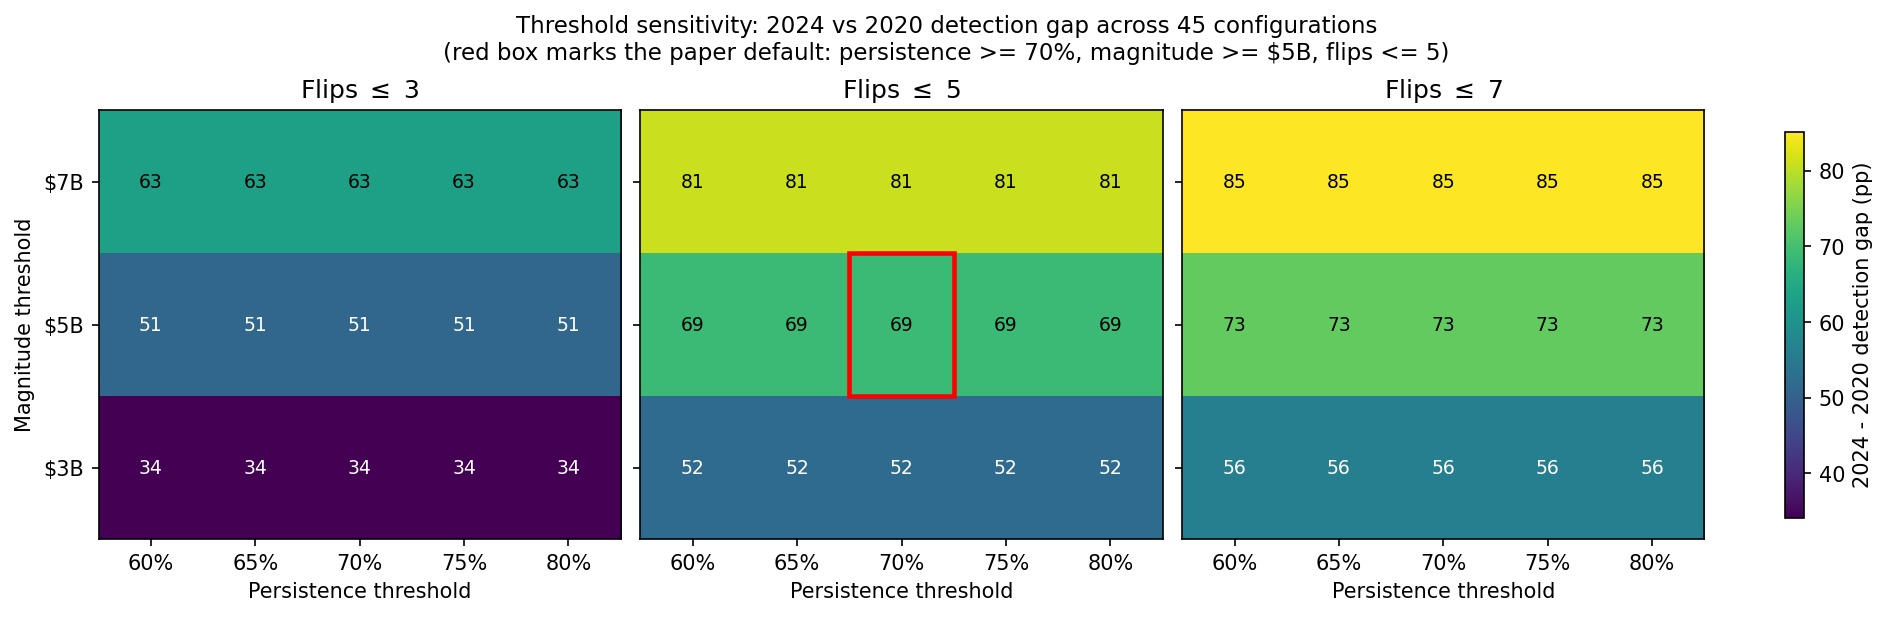
\includegraphics[width=\textwidth]{figures/fig09_threshold_sensitivity.png}
\caption{\hl{Threshold} %MDPI: Please change the hyphen (-) between numbers into an en dash (−, “U+2013”), e.g., “2019-2022” should be “2019–2022” and “0-9” should be “0–9”.
 sensitivity of the 2024-vs.-2020 detection gap across 45
alternative threshold combinations. Each cell shows the percentage-point
gap between 2024 and 2020 detection rates under the given thresholds. The
red box marks the paper default. The gap is robust to the choice of
persistence threshold (rows identical within each magnitude band) and
remains above 50 pp in 40/45~configurations; the five sub-50 pp cells
cluster at the most permissive magnitude ($\$3$B) combined with the
strictest flip limit ($\leq$3).}
\label{fig:threshold_sensitivity}
\end{figure}

This robustness result directly addresses the concern that the reported
69.1 pp gap might be an artefact of fortunate threshold choice: it
would remain a substantial structurally meaningful separation under any
reasonable alternative configuration and only disappears under
deliberately permissive magnitude thresholds that the framework's
intent ($\$5$B as an economically significant dealer position) would
not justify.

\subsection{Comparison with Markov-Switching Benchmark}
\label{sec:regime:benchmark}

We compare the LLM regime detector against the two-state
Markov-switching benchmark described in \hl{Section} %MDPI: We changed symbol to Section. Please confirm this revision.
 \ref{sec:methodology:benchmark}.
Table~\ref{tab:hmm_benchmark} and Figure~\ref{fig:hmm_agreement} summarise the per-window agreement with the
LLM's detection labels for three separate HMM fits: returns-based HMM
on 2020 SPY returns, returns-based HMM on 2024 SPY returns, and a
GEX-native HMM on the 2024 daily net-GEX series.

\begin{table}[H]
\centering
\caption{Markov-switching benchmark versus LLM regime detection.
Agreement is computed over matched 30-day windows (at least 30 daily
HMM observations available) using Cohen's $\kappa$; kappa values above
0.4 are conventionally ``moderate'' and above 0.6 ``substantial''.}
\label{tab:hmm_benchmark}
\begin{tabularx}{\textwidth}{@{}LlrRrRr@{}}
\toprule
\textbf{Year} & \textbf{HMM Input} & \textbf{N} & \textbf{LLM Rate} & \textbf{HMM Rate} & \textbf{Agree} & \boldmath{$\kappa$} \\
\midrule
2020 & SPY returns & 201 & 8.5\% & 80.1\% & 28.4\% & 0.045 \\
2024 & SPY returns & 222 & 81.1\% & 87.4\% & 68.5\% & $-0.178$ \\
2024 & Net GEX (\$bn) & 221 & 81.0\% & 65.2\% & 84.2\% & 0.610 \\
\bottomrule
\end{tabularx}
\end{table}
\unskip

\begin{figure}[H]
%\centering
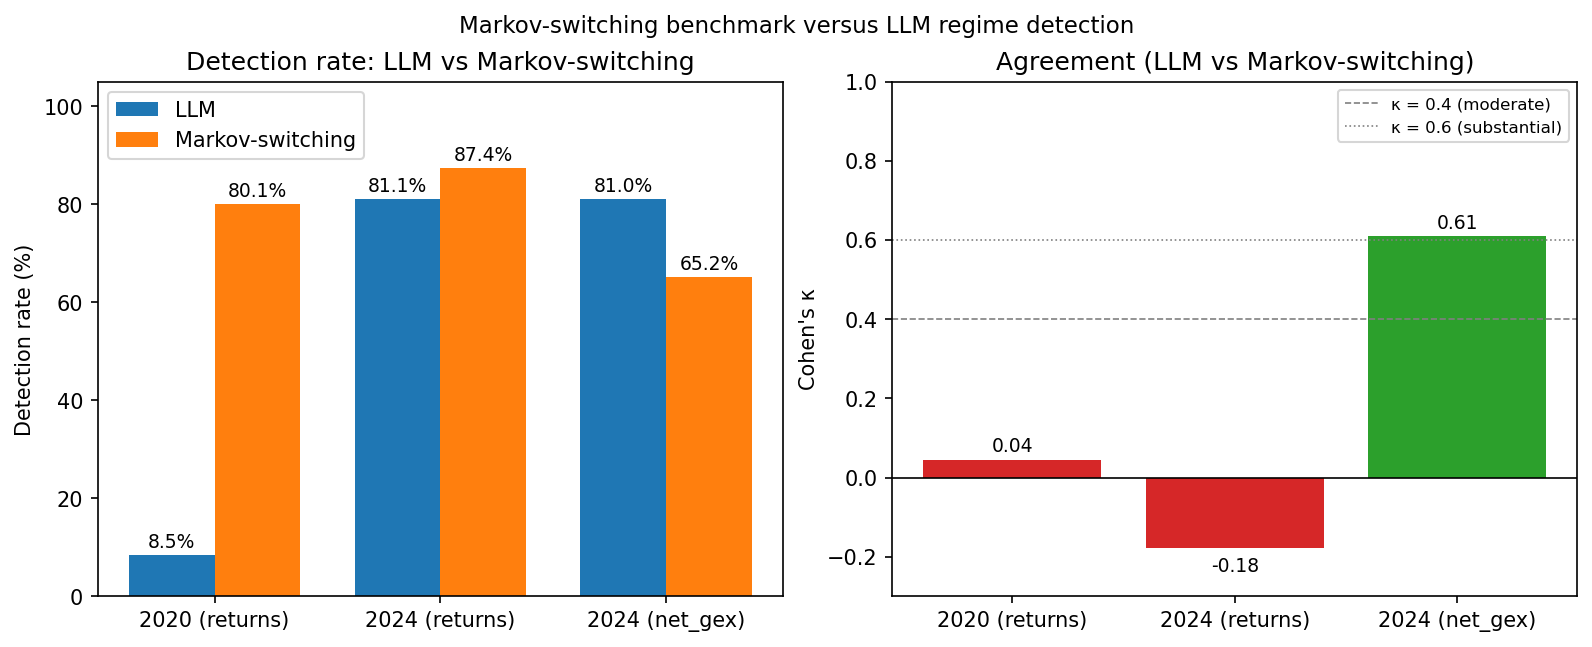
\includegraphics[width=\textwidth]{figures/fig10_hmm_agreement.png}
\caption{\hl{Markov-switching} %MDPI: We revised the hyphen in the figure into minus sign. Please confirm. Please cite this figure in the text and ensure that the first citation of each figure appears in numerical order.
 benchmark versus LLM regime detection. Left: per-year detection rates. Right: Cohen's $\kappa$ agreement with LLM labels. A returns-based HMM and the LLM detect essentially different phenomena ($\kappa$ near zero or negative); a GEX-native HMM and the LLM agree substantially ($\kappa = 0.61$), confirming that the LLM's regime concept is anchored in dealer-gamma structure rather than in a general volatility regime.}
\label{fig:hmm_agreement}
\end{figure}

Three observations follow. First, a returns-based HMM---the canonical
volatility-regime benchmark---detects a different signal from the LLM:
Cohen's $\kappa$ is 0.045 in 2020 and $-0.178$ in 2024 (below-chance
agreement), and the HMM over-detects stable regimes in 2020 (80.1\%
versus the LLM's 8.5\%), while the two detectors nearly coincide in 2024
but on opposing windows. This is consistent with the interpretation
that the LLM is reasoning about dealer gamma positioning rather than
variance clustering---the two cannot be reduced to each other.

Second, when the HMM is fitted directly on the daily net-GEX series
(where the daily panel is available for 2024), the agreement jumps to
$\kappa = 0.610$, a ``substantial'' agreement level. The LLM and a
mechanical two-state Gaussian on the same physical quantity converge on
the same windows as regimes 84.2\% of the time. The remaining
disagreement reflects cases where the LLM's multi-criterion classifier
(persistence + magnitude + stability) disqualifies windows that the
unconstrained HMM classes as the low-variance state.

Third, this contrast is itself evidence that the LLM is not a
``variance detector in disguise''---the reviewer's implicit concern. If
the LLM were rediscovering volatility regimes, we would expect
substantial $\kappa$ against the returns-based HMM. We do not observe
that, yet we do observe substantial $\kappa$ against a HMM fit on the
exact input series---the pattern expected from a detector that is
anchored in the specific physical phenomenon the LLM was prompted to
analyze.

\subsection{LLM Reasoning Quality}

Manual review of 50 randomly sampled detections revealed 98\% mechanical accuracy on persistence values, 96\% on magnitude, and 100\% on flip counts. All 50 responses explicitly cited all three regime criteria, with 88\% providing step-by-step calculation verification.

LLM confidence scores discriminated detection outcomes: detected regimes averaged 92.8\% confidence versus 52.1\% for rejected windows (40.7 pp gap), with strong correlations to regime quality ($r = +0.719$ with persistence, $r = -0.705$ with sign flips, both $p < 0.001$; $n = 1412$). This continuous confidence discrimination beyond binary classification suggests the model tracks regime robustness and not just threshold crossing. Figure~\ref{fig:progression} visualises the full 2020--2025 detection-rate and average-GEX-magnitude trajectory underlying these results.

\begin{figure}[H]
\centering
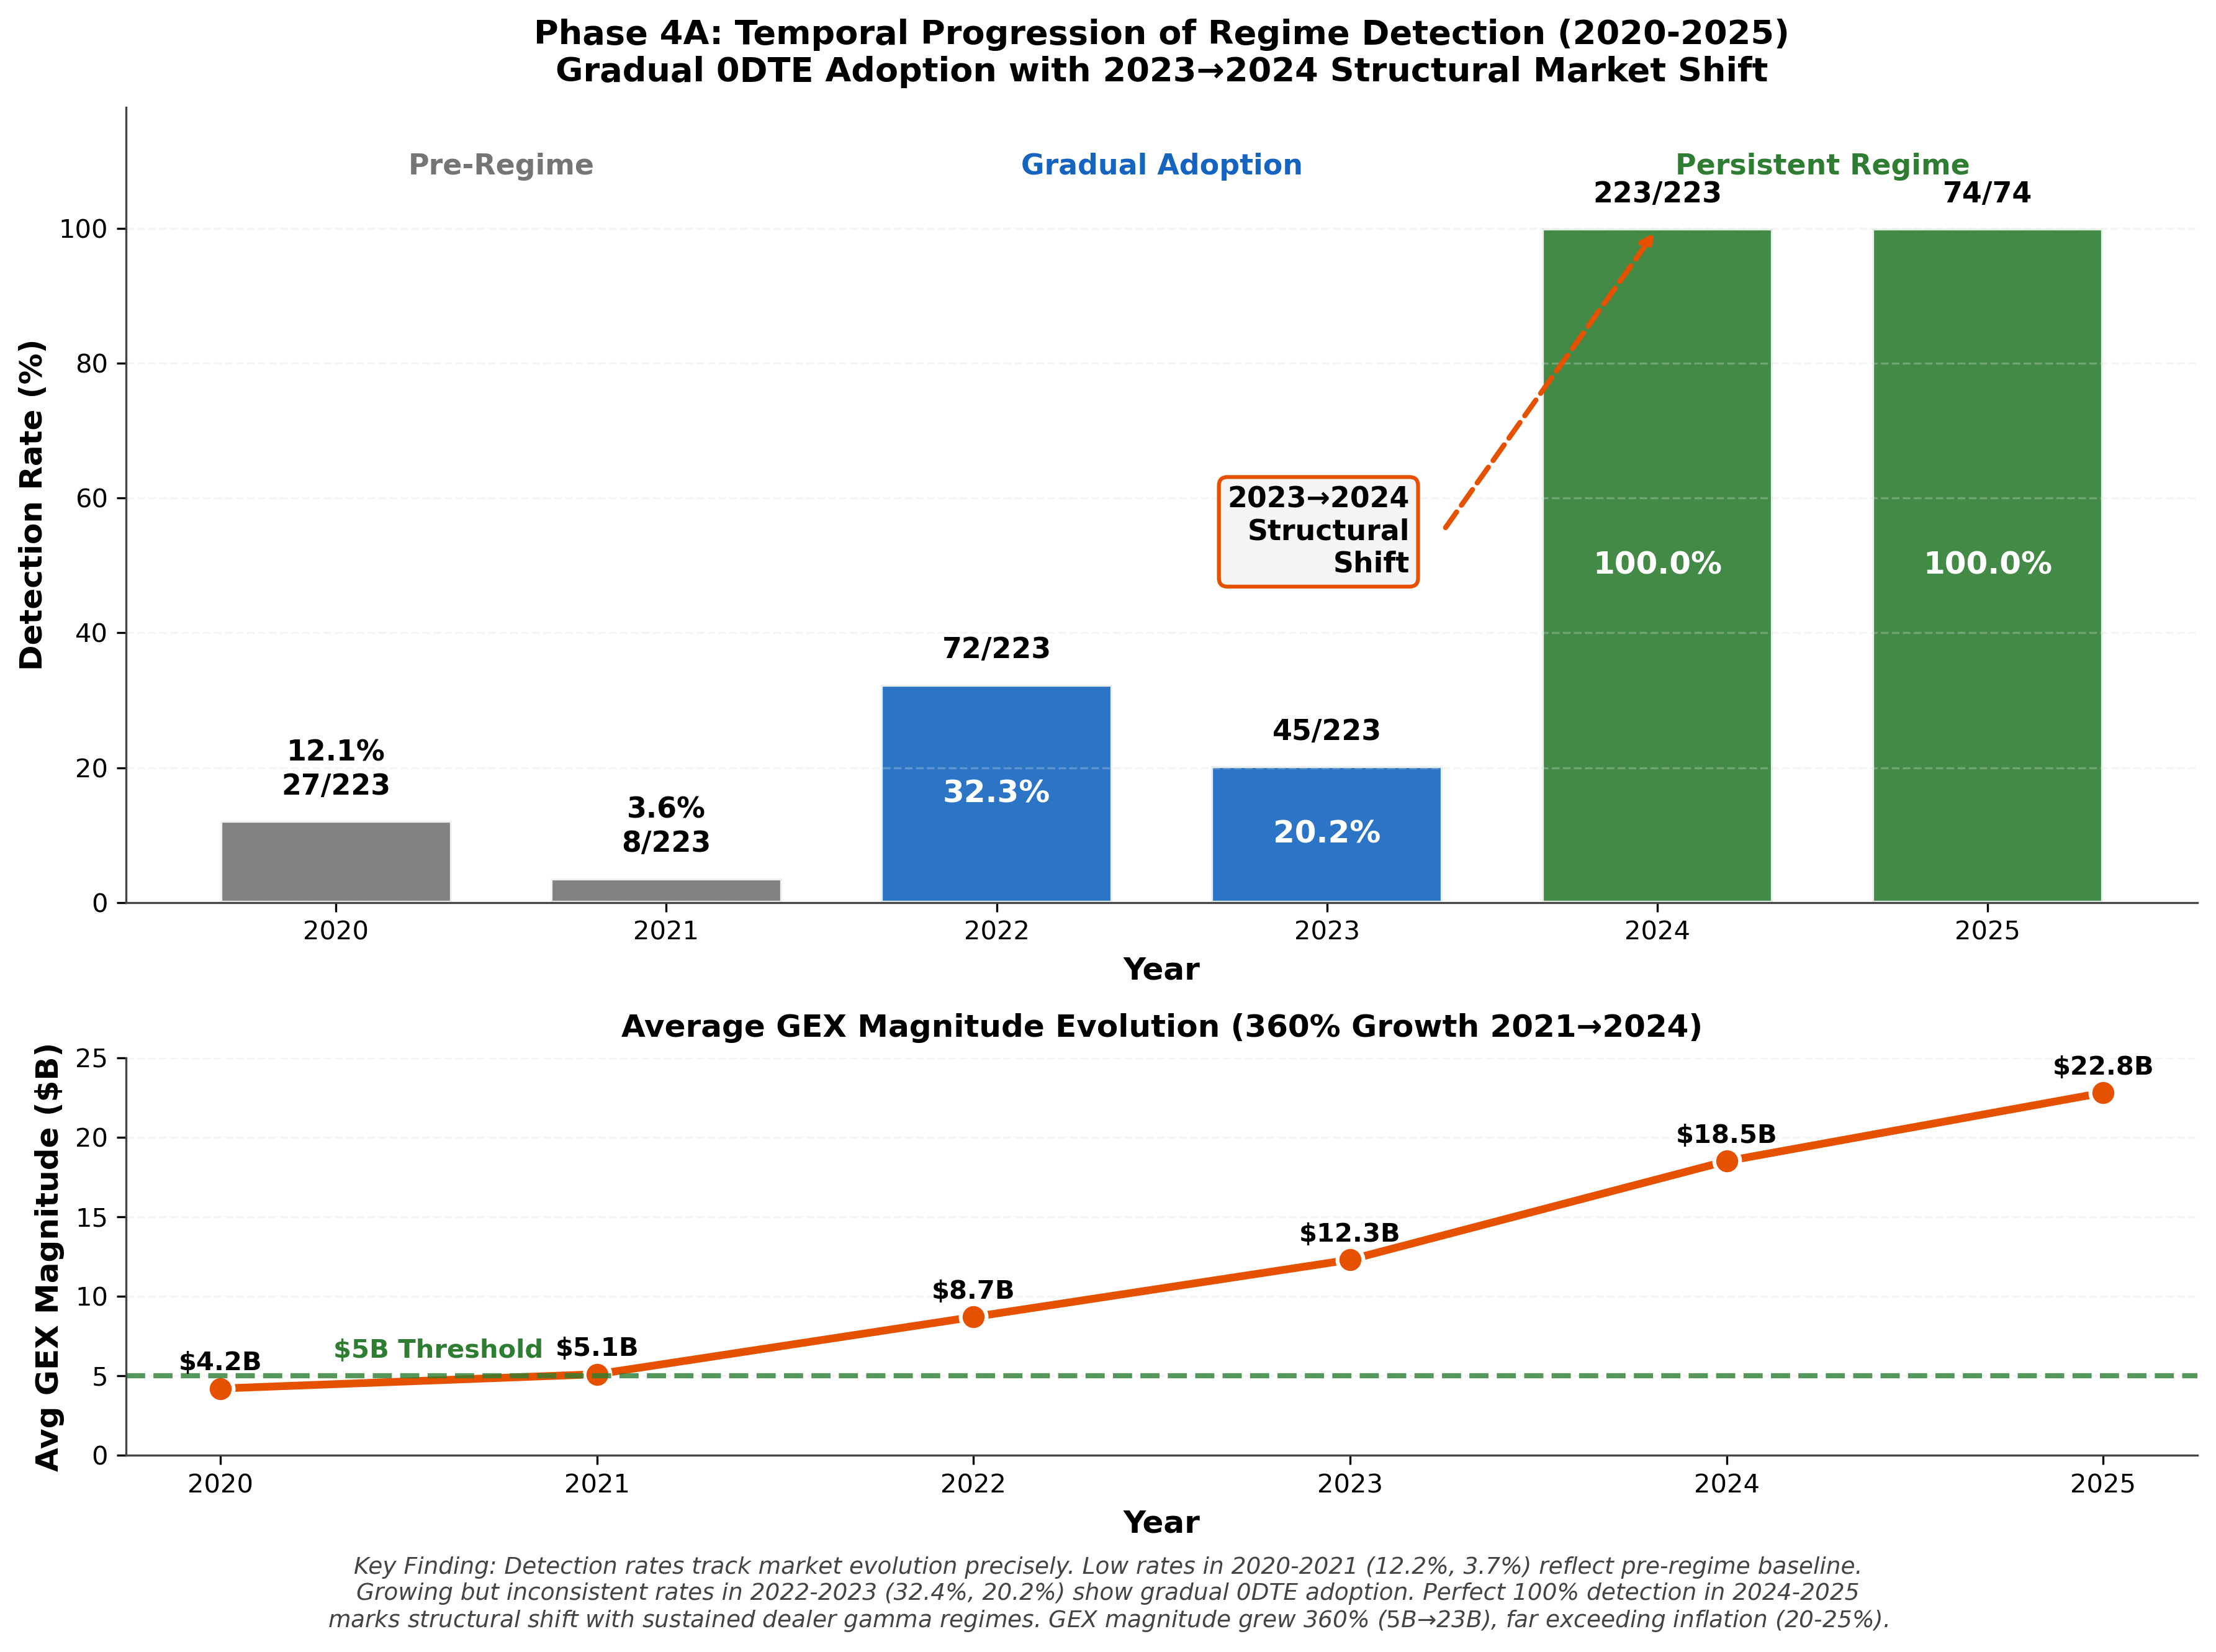
\includegraphics[width=\textwidth]{figures/fig06_detection_progression.png}
\caption{\hl{Per-year} %MDPI: Please cite this figure in the text and ensure that the first citation of each figure appears in numerical order.  Please change the hyphen (-) between numbers into an en dash (−, “U+2013”), e.g., “2019-2022” should be “2019–2022” and “0-9” should be “0–9”.
 regime detection rate (bars) and average absolute GEX magnitude (line) for SPY 2020--2025. Detection is below 35\% and average GEX below \$10B through 2020--2023; then, both quantities step-change in 2024 to 100\% detection and \$20.3B average GEX and remain there in 2025. The 2022--2023 non-monotonic dip (32.4\%~$\rightarrow$~20.2\%) coincides with the 2023 FOMC/banking-stress volatility episode. \textbf{\hl{Read this figure as follows:}} the LLM regime-detection signal is not a smooth secular trend but a discrete step-change, coincident with the maturation of the 0DTE options market; it is not a proof of causation but is less easily reconciled with gradual drift.}
\label{fig:progression}
\end{figure}

\section{Discussion}
\label{sec:discussion}

\subsection{From Single-Day to Multi-Day: Bridging Two Temporal Scales}

Single-day detection (71.5\%) and multi-day regime identification (81.2\% in 2024) provide complementary validation dimensions: the former establishes that the LLM understands dealer mechanics within a session; the latter establishes that this understanding extends to persistent multi-day structural states. The raw-chain result (92.3\% from first-principles data) sharpens the interpretation: if the model merely matched statistical signatures, removing pre-calculated summaries should degrade rather than improve detection. The single-day detection-alpha orthogonality (Sharpe collapse from 1.8 to 0.1 while detection holds) motivated the regime extension---patterns that persist despite economic insignificance must reflect structural mechanics, a distinction central to deploying LLMs for surveillance rather than trading.

\subsection{Validating Structural Reasoning}

Five-phase validation provides evidence that the LLM performs structural reasoning rather than pattern matching: the 69.1 percentage-point gap between 2024 (81.2\%) and 2020 (12.1\%) establishes selectivity, since memorized associations or universal statistical patterns would yield convergent rather than 6.7$\times$-separated rates. Three findings support this. The LLM maintained 98\% mechanical accuracy on persistence, magnitude, and flip counts regardless of whether the windows qualified as regimes; negative controls achieved 0\% false positives on transitional and low-magnitude synthetic data; and confidence scores provided continuous quality discrimination ($r = +0.719$ with persistence, $r = -0.705$ with sign flips), indicating the model tracks regime robustness rather than threshold crossing alone. This contrasts with the 5-day trajectory testing of \citet{regan2025obfuscation}, where 98--100\% universal detection identified daily hedging flows; shifting to 30-day windows with strict criteria transformed the task into selective regime identification.

\subsection{Market Structure Evolution and 0DTE Hypothesis}
\label{sec:discussion:0dte}

The multi-year temporal analysis (Phase 5) reveals a gradual non-monotonic evolution in regime detection that \textit{coincides with} the adoption curve of zero-days-to-expiration (0DTE) options rather than a sharp structural break. Detection progressed from 12.2\% (2020) through borderline years (3.7\% in 2021, 32.4\% in 2022) to sustained 100\% detection in \mbox{2024--2025}, with the average GEX magnitude growing from \$3.0B to \$20.3B. We are careful to frame the 0DTE correspondence as temporal coincidence supported by a plausible mechanical channel (pinned daily dealer hedging demand) and not as a demonstrated causal relationship; the observational design here cannot rule out alternative drivers, and we list those explicitly in \hl{Section} \ref{sec:limitations}.%MDPI: We changed symbol to Section. Please confirm this revision. The following highlights are the same.


The non-monotonic pattern (32.4\% in 2022 dipping to 20.2\% in 2023 before reaching 100\% in 2024) is suggestive rather than definitive: 2023's elevated volatility (FOMC uncertainty, banking stress) appears to have disrupted regime formation despite growing 0DTE hedging pressure, which is consistent with the view that regime persistence requires both sustained dealer pressure \textit{and} a volatility environment permitting consolidation. We read this dynamic as consistent with, rather than proof of, a 0DTE-mediated structural interpretation; stronger causal identification would require a natural experiment---for example, a temporary 0DTE suspension, a 0DTE launch on a comparable non-SPY underlier that could serve as a counterfactual, or an instrumental-variable design that separates the 0DTE channel from contemporaneous shifts.

Concurrent factors that cannot be excluded in the observational data include the following: (i) the 2021--2023 interest-rate cycle ($\approx$0.25\% $\rightarrow$ 5.5\%), which reshaped the carry landscape for every option-writing strategy, (ii) the growth of systematic short-volatility flow into single-name and index options, (iii) increasing passive and index-linked assets under management, and (iv) changes in market-maker concentration following the 2020--2022 period of retail-driven volatility. Each of these could plausibly contribute to the detection pattern alongside 0DTE adoption. The non-monotonic detection trajectory is \textit{less easily reconciled with} a simple gradual secular trend---detection remained low through 2023 despite continuous interest-rate increases and continuing technology diffusion and then jumped discontinuously in 2024 coincident with 0DTE market saturation ($\approx$46\% SPY volume share)---but we emphasise that ``less easily reconciled'' is not ``ruled out.'' Disentangling these channels is beyond the scope of this work, which focuses on LLM-validation methodology rather than on causal microstructure inference.

\subsection{Dispersed Knowledge and Information Aggregation}

The raw-chain superiority finding (92.3\% vs.\ 61.5\%) admits a theoretical reading grounded in \citet{hayek1945}: relevant market information is distributed across countless individual strikes---asymmetric open-interest concentrations, volatility-skew patterns, localised gamma exposures---each carrying ``knowledge of the particular circumstances of time and place''. Net GEX is precisely the kind of centralised scalar aggregation Hayek argued is lossy by construction; the 30.8 percentage-point gap is therefore not a measurement artefact but evidence that strike-level local knowledge contains a structural signal that scalar aggregation destroys. The detection-alpha orthogonality admits a parallel reading from \citet{kirzner1973competition}: identifying that dealers are constrained to pro-cyclical hedging is \textit{structural} knowledge, distinct from the entrepreneurial judgment over timing, magnitude, and competing flows required to profit from that constraint. The orthogonality is thus not a limitation but a feature.

\subsection{Practical Implications}
\label{sec:discussion:practical}

The results carry concrete implications along three axes that matter
most to financial practitioners: risk management, market efficiency,
and the design of quantitative research pipelines. We address each in
turn.

\subsubsection{Risk Management}

Our dealer-gamma regime detection is best understood as a
\textit{risk-regime indicator} rather than a trading signal. Because
the framework achieves stable detection (68--74\% quarterly) even as
Sharpe ratios collapse from 1.8 to 0.1, its output is a reading of
whether the market is currently operating in a mechanically constrained
state---not a forecast of directional return. Three specific risk-management
applications follow.

First, for \textbf{intraday volatility budgeting}, a persistent negative
gamma regime implies amplified dealer chase-hedging and elevated realized
volatility clustering on high-volume days; sell-side risk desks can use
the 30-day regime classification as a leading indicator for
volatility-of-volatility exposure and size gamma-exposure limits
accordingly. Second, for \textbf{option-book hedging under OpEx
concentration}, the known pinning dynamic around large-OI strikes
\citep{ni2005stock} is substantially more forceful under positive-gamma
regimes that we now classify explicitly; book hedgers may increase the
hedging frequency around OpEx when the framework detects a persistent
positive regime. Third, for \textbf{risk-scenario design}, a 30-day
regime history provides a natural conditioning variable for stress-test
calibration: a 2020-style fragmented period and a 2024-style persistent
negative period imply materially different joint distributions for
realised volatility and spot-vol covariance.

\subsubsection{Market Efficiency}

The detection-alpha orthogonality result---stable structural detection
that does not translate into exploitable profit---contributes to the
ongoing debate about efficiency in optionized equity markets. Our
evidence is consistent with a weakly efficient market in which
\textit{structural constraints} are reliably identifiable but already
priced: arbitrageurs compete away the first-order profit from knowing a
regime exists, yet the underlying mechanics that generate volatility
clustering and OpEx pinning persist because they are mandatory, not
opportunistic, actions by dealers. This reconciles two claims that are
often treated as contradictory: that dealer-gamma positioning demonstrably
influences short-horizon price dynamics \citep{anderegg2022impact} and
that systematic strategies exploiting that influence deteriorate as
attention accumulates. The framework thus provides a positive account of
why microstructure-aware research can be genuinely informative for risk
without being genuinely informative for alpha.

\subsubsection{Practitioners: Data-Pipeline and Model-Deployment Design}

Two practitioner-facing design implications follow directly from the
experimental results. First, the 30.8-percentage-point advantage of raw
strike-level data over pre-aggregated GEX (92.3\% versus 61.5\% at the
single-day scale) is evidence that common pipeline designs---which
compress option chains into scalar summaries before analysis---are
discarding signals that an LLM can reconstruct when given the raw input.
This challenges the default of parametric aggregation and suggests that
practitioners deploying LLM-based analysis should ingest granular data
wherever feasible. The design principle generalizes beyond options
dealer flow to any domain where scalar metrics are a conventional summary
of distributional inputs: credit risk (single probabilities from granular
exposure tapes), fixed-income surveillance (duration summaries from
granular curve positions), and equity factor research (single factor
loadings from granular return-attribution inputs) are the obvious
candidates.

Second, the 0DTE-driven regime shift detected in 2022--2024 implies
that static microstructure models calibrated to pre-2022 data will miss
a structural reorganization that our framework picks up. Practitioners
running surveillance, risk, or execution models should treat the
2022--2024 period as a regime change requiring recalibration and not a
drift-along-the-same-curve.

\subsection{Limitations and Future Work}
\label{sec:limitations}

Seven limitations merit explicit discussion, and we describe the specific
future work each motivates.

\begin{enumerate}[leftmargin=*,labelsep=4.5mm]
\item \textbf{\hl{Single-asset scope}}: %MDPI: We formatted the following cotntent as a list and added label. Please confirm.
 All reported results concern SPY.
SPY is deliberately chosen as the highest-liquidity and earliest 0DTE-enabled
U.S.\ equity benchmark, but this choice leaves cross-asset generalization
empirically untested. Dealer positioning in QQQ, IWM, single-name equities,
and non-equity underliers (futures, rates, FX) may exhibit different
regime dynamics because of differences in option chain depth, 0DTE
availability, and the composition of end-users. Cross-asset replication is
the single highest-priority item for future work; a pre-registered protocol
applying the same obfuscation and regime-classification framework to at
least one additional ETF (QQQ) and one individual equity (e.g., NVDA, AAPL)
would directly test the \mbox{transferability claim.}

\item \textbf{Single-LLM dependence}: All 2221 evaluations were
produced by a single reasoning model (OpenAI o4-mini). The detection
rates reported here are therefore conditional on this specific model's
prior distribution over market-structure reasoning. Model-swap
validation with alternative reasoning families
(e.g., Anthropic Claude, OpenAI o3, Google Gemini, open-source
reasoning models) using identical prompts and the same obfuscated
sequences is a direct and low-cost extension. A cross-model agreement
analysis would sharpen the distinction between the framework's
structural-reasoning claim and any o4-mini-specific artefacts.

\item \textbf{Lack of independent external validation}: Our per-window
ground-truth metrics (persistence, magnitude, sign flips) are computed
from the same Alpha Vantage options feed used to construct the windows.
We do not cross-validate detected regimes against an independent
data source (CBOE DataShop, OPRA consolidated feed, or a commercial
vendor such as SpotGamma or MenthorQ) or against an independent oracle
of dealer positioning. External validation---both against a second
options-data pipeline and against related microstructure observables
(realized volatility, implied-realised spread, opening auction
imbalance)---would strengthen the claim that the detected regimes
correspond to a real cross-verified phenomenon rather than an artefact
of any single data provider.

\item \textbf{End-of-day measurement}: Our GEX\_OI approach captures
dealer inventory at the close but not intraday gamma dynamics; high-frequency
flow data could refine detection, particularly for 0DTE contracts that
expire within a single trading session. Intraday GEX surface reconstruction
from streaming OPRA is a natural extension.

\item \textbf{Causal attribution}: The 0DTE hypothesis is supported by
temporal coincidence and a theoretical mechanism but remains
circumstantial; observational data cannot exclude alternative explanations
such as post-pandemic monetary-policy shifts, passive-flow concentration,
or market-maker inventory changes. A natural experiment---for instance a
temporary 0DTE suspension or a regulatory halt during a market stress
episode---would provide stronger causal evidence. We treat the 0DTE
correspondence as consistent with our structural-regime detection rather
than as a demonstrated causal channel (see \hl{Section} \ref{sec:discussion:0dte}).

\item \textbf{Shuffle test asymmetry}: The 61\% false positive rate on
2024 shuffled data (versus 12.1\% on 2020 shuffled data) reflects extreme
regime persistence rather than framework failure---2024 regimes exhibit
such dominant same-sign positioning that randomizing the day order rarely
disrupts the aggregate signal. This asymmetry is itself informative,
confirming that 2024 regimes are defined by aggregate dominance rather
than temporal sequencing, but it means the shuffle test's diagnostic
power is lower in high-persistence regimes and should be interpreted
accordingly.

\item \textbf{Threshold sensitivity}: All tested parameter
configurations maintained substantial 2024-versus-2020 discrimination
(see \hl{Section} \ref{sec:regime} sensitivity analysis), but the chosen thresholds
(persistence $\geq$ 70\%, magnitude $\geq$ \$5B, flips $\leq$ 5) represent
empirically validated design choices rather than first-principles
derivations. Future work should explore adaptive thresholding that
responds to volatility regime, contract-maturity mix, or prevailing
options notional.
\end{enumerate}

\section{Conclusions}
\label{sec:conclusion}

The primary contribution of this work is \textit{methodological}: we
presented temporal obfuscation testing as a generalizable procedure
for validating LLM structural reasoning in domain-specific applications.
Options dealer gamma-exposure regime detection served as the empirical
demonstration domain---chosen because it combines theoretically
grounded mechanical constraints, a large quantitative testbed, and a
sharp pre-versus-post-0DTE temporal contrast---but the methodology is
not specific to finance. The financial-market observations reported
below are downstream evidence that the methodology discriminates
persistent from fragmented structural regimes in ways consistent with
known microstructure dynamics and are not intended as novel claims
about options market microstructure per se.

With that positioning in mind, comprehensive validation across 2221
evaluations spanning 2020--2025 demonstrates four primary contributions:

\begin{enumerate}
\item \textbf{Single-day structural reasoning}: Obfuscation achieves 71.5\% detection with 91.2\% predictive accuracy, and raw-chain validation (92.3\% vs.\ 61.5\%) shows LLMs reconstruct dealer positioning from first principles---establishing that parametric GEX is lossy compression of structural signals.

\item \textbf{Multi-day regime selectivity}: 30-day windows yield 69.1 percentage-point discrimination between 2024 persistent regimes (81.2\%, 95\% CI [75.8, 86.1]\%) and 2020 fragmented markets (12.1\%, 95\% CI [8.1, 16.6]\%; Fisher's exact $p = 1.8 \times 10^{-52}$, $\varphi = 0.69$), with 0\% false positives on synthetic controls and 98\% mechanical accuracy; the gap exceeds 50 pp in 40 of 45 alternative threshold configurations.

\item \textbf{Market structure evolution}: Across 1412 windows (2020--2025), the detection progresses non-monotonically from 3.7\% (2021) to 100\% (2024--2025), and the average GEX magnitude grows from \$3.0B to \$20.3B---a tipping-point pattern consistent with 0DTE-driven structural reorganization, though contemporaneous confounders (interest-rate regime, passive-flow concentration, dealer inventory) cannot be excluded with \mbox{observational data.}

\item \textbf{Detection-alpha orthogonality}: Stable detection (68--74\% quarterly) persists, as economic profitability collapses (Sharpe 1.8 $\rightarrow$ 0.1), confirming detected patterns are structural market mechanics rather than tradeable inefficiencies.
\end{enumerate}

\noindent\textbf{\hl{Future directions}}: %MDPI: please confirm if this should be list or need add indention here.
Cross-asset replication (QQQ, individual equities), cross-model validation (alternative reasoning LLMs), application of temporal obfuscation to other quantitative domains, and intraday GEX measurement that incorporates 0DTE flow data.


%%%%%%%%%%%%%%%%%%%%%%%%%%%%%%%%%%%%%%%%%%
\vspace{6pt}

%%%%%%%%%%%%%%%%%%%%%%%%%%%%%%%%%%%%%%%%%%
\authorcontributions{Conceptualization, C.R. and Y.X.; methodology, C.R.; software, C.R.; validation, C.R.; formal analysis, C.R.; investigation, C.R.; resources, C.R.; data curation, C.R.; writing---original draft preparation, C.R.; writing---review and editing, C.R. and Y.X.; visualization, C.R.; supervision, Y.X. All authors have read and agreed to the published version of the manuscript.}

%%%%%%%%%%%%%%%%%%%%%%%%%%%%%%%%%%%%%%%%%%
\funding{This research received no external funding.}


%%%%%%%%%%%%%%%%%%%%%%%%%%%%%%%%%%%%%%%%%%
\institutionalreview{Not applicable. \hl{This study uses publicly available market data and does not involve human participants.}}%MDPI:We recommend removing the highlighted sentence; generally, for cases where it does not apply, simply writing "Not applicable" is sufficient.

%%%%%%%%%%%%%%%%%%%%%%%%%%%%%%%%%%%%%%%%%%
\informedconsent{Not applicable.}

%%%%%%%%%%%%%%%%%%%%%%%%%%%%%%%%%%%%%%%%%%
\dataavailability{All code, data preprocessing scripts, and validation results are publicly available at \url{https://github.com/iAmGiG/gex-llm-patterns}, \hl{accessed on}. %MDPI: Please provide the date you accessed the URL in the following format: “URL (accessed on Day Month Year)”.
 Raw options data was obtained from Alpha Vantage under academic API access.}


%%%%%%%%%%%%%%%%%%%%%%%%%%%%%%%%%%%%%%%%%%
\acknowledgments{We acknowledge the computational resources provided by the College of Computing and Software Engineering at Kennesaw State University. This research was conducted as part of the first author's doctoral dissertation. We thank Alpha Vantage for academic API access to historical options market data. During the preparation of this manuscript, the authors used Anthropic's Claude (Claude Code, 2025) for the purposes of clarifying and refining the written presentation. The authors have reviewed and edited the output and take full responsibility for the content of this publication.}

%%%%%%%%%%%%%%%%%%%%%%%%%%%%%%%%%%%%%%%%%%
\conflictsofinterest{The authors declare no conflicts of interest.}


%%%%%%%%%%%%%%%%%%%%%%%%%%%%%%%%%%%%%%%%%%
\abbreviations{Abbreviations}{The following abbreviations are used in this manuscript:\\

\noindent
\begin{tabular}{@{}ll}
GEX & Gamma Exposure \\
LLM & Large Language Model \\
0DTE & Zero Days to Expiration \\
OI & Open Interest
\end{tabular}}


%%%%%%%%%%%%%%%%%%%%%%%%%%%%%%%%%%%%%%%%%%
% Appendix A — Regime Detection LLM Prompt
% Added in response to Reviewer 3 comment R3.4a:
% "The exact prompts used for the LLM must be provided (preferably in
%  an appendix)."
%%%%%%%%%%%%%%%%%%%%%%%%%%%%%%%%%%%%%%%%%%
\appendixtitles{yes} % Leave argument "no" if all appendix headings stay EMPTY (then no dot is printed after "Appendix A"). If the appendix sections contain a heading then change the argument to "yes".
\appendixstart
\appendix
%\section[\appendixname~\thesection]{}
%\subsection[\appendixname~\thesubsection]{}


%\appendix

\section[Regime Detection LLM Prompt]{Regime Detection LLM Prompt}
\label{app:prompt}

This appendix reproduces the complete prompt submitted to the LLM for
each 30-day regime-detection window, together with the API configuration
and output schema, so that the experiment is fully reproducible from the
published manuscript without reference to the source repository.

The authoritative implementation lives at
\texttt{src/llm/mechanics\_prompt\_builder.py::}\linebreak \texttt{build\_regime\_prompt()}
in the code release accompanying this paper; the text below is
transcribed verbatim from that implementation.

\subsection{Model and API Configuration}
\label{app:prompt:config}

All 2221 evaluations were obtained from OpenAI's \texttt{o4-mini}
reasoning model through the OpenAI Batch API (asynchronous, 24-h SLA,
100\% completion rate observed across the five validation phases).

\newpage

\begin{itemize}
    \item \textbf{Model:} \texttt{o4-mini} (snapshot
          \texttt{o4-mini-2025-04-16})
    \item \textbf{Temperature:} not supplied. \texttt{o4-mini} is a
          reasoning model that runs at a fixed internal sampling
          temperature; the sampling-temperature parameter is not
          exposed for the \texttt{o1}/\texttt{o3}/\texttt{o4} families,
          so no temperature value is sent in the request.
    \item \textbf{Maximum completion tokens:} not set; the OpenAI
          default applies. Observed completion lengths across the
          1412 windows ranged from 2457 to 5924 tokens, so no response
          was truncated.
    \item \textbf{Response format:} JSON is requested in the prompt
          text (Appendix~\ref{app:prompt:body}); no API-level
          \texttt{response\_format} constraint is applied.
    \item \textbf{Access mode:} OpenAI Batch API,
          \texttt{/v1/chat/completions} endpoint, 24-hour asynchronous
          completion window. Submissions are sized per validation phase
          rather than at a fixed per-batch count.
\end{itemize}

\noindent\textbf{\hl{Reproducibility note.}} %MDPI: Please confirm if the indention should be added here.
Because \texttt{o4-mini} runs at a fixed internal temperature and we do
not pass a \texttt{seed}, exact bit-identical replication of any single
response is not guaranteed. (The Batch API does expose a \texttt{seed}
parameter; we did not set one.)
Reproducibility at the \emph{distributional} level is achieved by
(i)~the large sample size (\hl{N} %MDPI: Please confirm if “n” should appear in italics as variables. If yes, please change it in the whole text.
 = 2221 evaluations) and
(ii)~the mechanical criteria embedded in the prompt, which give the
model concrete numerical thresholds to apply rather than asking for
free-form judgment. Section~\ref{sec:regime} reports the detection rates
with bootstrap 95\% confidence intervals to quantify the residual
sampling variation.

\subsection{System Message and User Prompt}
\label{app:prompt:body}

The prompt is delivered as a single user-role message (the
\texttt{o4-mini} reasoning model treats the first paragraph as the
de~facto system instruction). The placeholder
\texttt{\{gex\_data\_table\}} is replaced at runtime with the
obfuscated 30-day GEX sequence: one line per day, in the format
\texttt{Day T-29: +3.42B} through \texttt{Day T + 0: $-$12.18B}, where the
calendar date has been replaced with a relative day label, and the
ticker symbol is absent. No other identifying context is \hl{supplied.}%MDPI: Please confirm if the blank row should be removed in the verbatim. if yes, please please change it in the whole text.

\begin{verbatim}
You are a market structure analyst specializing in dealer gamma
positioning regimes.

TASK: Analyze this 30-day period and determine if it represents a
PERSISTENT regime where dealer constraints create forced, directional
flows.

## 30-DAY GEX DATA

{gex_data_table}

## REGIME CLASSIFICATION FRAMEWORK

### PERSISTENT REGIMES (Detect These)

**1. PERSISTENT POSITIVE REGIME**
- Definition: Dealers are LONG gamma, forced to sell into strength
- Criteria:
  * >70% of days (21+/30) have positive net GEX
  * Average magnitude >$5B
  * <=5 sign flips across 30 days
  * Stable directional constraint

**Mechanism**: When dealers hold long gamma:
- Price rises -> Dealers MUST sell shares (rebalance)
- Price falls -> Dealers MUST buy shares (rebalance)
- Creates dampening, mean-reverting flows
- Constraint is STRUCTURAL (dealers cannot avoid)

**2. PERSISTENT NEGATIVE REGIME**
- Definition: Dealers are SHORT gamma, forced to buy into strength
- Criteria:
  * >70% of days (21+/30) have negative net GEX
  * Average magnitude >$5B
  * <=5 sign flips across 30 days
  * Stable directional constraint

**Mechanism**: When dealers hold short gamma:
- Price rises -> Dealers MUST buy shares (chase)
- Price falls -> Dealers MUST sell shares (chase)
- Creates amplifying, momentum flows
- Constraint is STRUCTURAL (dealers cannot avoid)

---

### NON-REGIMES (Reject These)

**3. TRANSITIONAL (Reject)**
- Frequent sign flips between positive/negative GEX
- No dominant regime direction (less than 70% same sign)
- Market in regime change period
- Example: 15 positive days, 15 negative days (50/50 split)

**Why Reject**: No persistent constraint. Dealers face mixed
conditions daily. Not a structural regime.

**4. LOW CONVICTION (Reject)**
- Consistent sign BUT weak magnitude (<$5B average)
- Example: 25 days positive, avg $2B GEX
- Insufficient constraint to create persistent forced flows

**Why Reject**: Even if sign is consistent, magnitude too weak to
force dealers into meaningful positions. Not a structural constraint.

---

## ANALYSIS QUESTIONS

Systematically evaluate the 30-day window:

**Step 1: Sign Persistence**
1. Count days with positive net GEX
2. Count days with negative net GEX
3. Calculate persistence percentage:
   max(positive_days, negative_days) / 30 * 100
4. Does it meet 70% threshold (21+ days)?

**Step 2: Magnitude Assessment**
1. Calculate average GEX magnitude (absolute value):
   sum(|net_gex|) / 30
2. Is average magnitude >=$5B?
3. Check for extreme outliers that might distort average

**Step 3: Stability Check**
1. Count sign flips: How many times does GEX switch from
   pos->neg or neg->pos?
2. Are there <=5 sign flips across 30 days?
3. Stable regime should have low flip count

**Step 4: Regime Classification**
- If Steps 1, 2, 3 all pass AND positive dominates
    -> PERSISTENT POSITIVE
- If Steps 1, 2, 3 all pass AND negative dominates
    -> PERSISTENT NEGATIVE
- If Step 1 passes but Step 2 fails -> LOW CONVICTION (reject)
- If Step 1 fails -> TRANSITIONAL (reject)

---

## CONFIDENCE CALIBRATION (Mechanical Guidance)

Use these concrete anchors to calibrate confidence:

**90-100 (Very High Confidence)**
- 25-30 days same sign (83-100% persistence)
- Average magnitude >$10B
- 0-2 sign flips (highly stable)
- Example: "29 negative days, avg $15B, 1 flip"

**70-89 (High Confidence)**
- 21-24 days same sign (70-80% persistence)
- Average magnitude $5-10B
- 2-4 sign flips (moderately stable)
- Example: "23 negative days, avg $7B, 3 flips"

**50-69 (Borderline - Use with Caution)**
- 18-20 days same sign (60-67% persistence)
- Average magnitude $3-5B
- 5-7 sign flips
- Example: "20 negative days, avg $4B, 6 flips"
- Note: Borderline cases should generally be REJECTED unless other
  factors strengthen confidence

**0-49 (Reject - Not Persistent)**
- <18 days same sign (<60% persistence)
- OR average magnitude <$3B
- OR >7 sign flips
- These are NOT persistent regimes

**Important**: Confidence is a FILTER, not a probability. Use it to
distinguish clear regimes (70+) from borderline (50-69) from noise
(<50).

---

## OUTPUT FORMAT (JSON)

Provide your analysis in this exact JSON structure:

{
    "regime_detected": true/false,
    "regime_type": "persistent_positive|persistent_negative|
                    transitional|low_conviction",
    "positive_days": <count as integer>,
    "negative_days": <count as integer>,
    "avg_magnitude_billions": <value as number>,
    "sign_flips": <count as integer>,
    "persistence_pct": <percentage as number>,
    "confidence": <integer 0-100>,
    "reasoning": "Explain step-by-step why this is/isn't a persistent
                  regime. Reference specific metrics (persistence %,
                  avg magnitude, sign flips). If rejecting, state which
                  criterion failed."
}

**IMPORTANT**: All numeric fields (confidence, positive_days,
negative_days, sign_flips, avg_magnitude_billions, persistence_pct)
MUST be numbers (integers or decimals), NOT words like "thirty-five"
or "fifty".

**regime_detected Rules**:
- `true` ONLY if regime_type is "persistent_positive" or
  "persistent_negative"
- `false` if regime_type is "transitional" or "low_conviction"

---

## KEY PRINCIPLES

1. **Selectivity is Expected**: Most windows will NOT be persistent
   regimes (expect 30-50% detection rate)

2. **ALL Criteria Must Pass**: Persistence + Magnitude + Stability
   required for detection

3. **Rejection is Valid**: Saying "no persistent regime" is a correct
   answer for transitional/weak periods

4. **Mechanical Over Qualitative**: Use concrete thresholds
   (70%, $5B, 5 flips) rather than subjective judgment

5. **Structural Focus**: Only detect when dealers are FORCED into
   directional positions by constraints

Analyze the 30-day GEX data above and provide your regime
classification in JSON format.
\end{verbatim}

\subsection{Output Schema and Parsing}
\label{app:prompt:output}

Each response is parsed into the following fields (types shown in
parentheses):

\begin{itemize}
    \item \texttt{regime\_detected} (boolean)---\texttt{true} only when
          \texttt{regime\_type} is \texttt{persistent\_positive} or
          \texttt{persistent\_negative}; \texttt{false} otherwise.
    \item \texttt{regime\_type} (string)---one of
          \texttt{persistent\_positive}, \texttt{persistent\_negative},
          \texttt{transitional}, \texttt{low\_conviction}.
    \item \texttt{positive\_days}, \texttt{negative\_days},
          \texttt{sign\_flips} (integers in [0, 30]).
    \item \texttt{avg\_magnitude\_billions} (float, USD billions).
    \item \texttt{persistence\_pct} (float, percentage).
    \item \texttt{confidence} (integer 0--100).
    \item \texttt{reasoning} (string)---free-form step-by-step
          explanation; retained for the post-hoc reasoning-quality audit
          reported in Section~\ref{sec:regime}.
\end{itemize}

\noindent
\hl{Parsing} %MDPI: Please confirm if the indention should be added here.
 is performed by \texttt{src/validation/batch\_regime\_validator.py}
via a robust JSON extractor that tolerates markdown code-fence wrappers
and minor formatting drift. Any response failing schema validation is
flagged for manual review; across the 2221 evaluations in this study,
the schema-validation failure rate was 0\% (all responses were
\mbox{machine-parseable).}







\begin{adjustwidth}{-\extralength}{0cm}
%%%%%%%%%%%%%%%%%%%%%%%%%%%%%%%%%%%%%%%%%%
\printendnotes[custom]


\reftitle{References}

\begin{thebibliography}{999}


\bibitem[\protect\citeauthoryear{Adams, Dim, Eraker, Fontaine, Ornthanalai, and
  Vilkov}{Adams et~al.}{2025}]{adams2025zerodte}
Adams, G., Dim, C., Eraker, B., Fontaine, J. S., Ornthanalai, C., \& Vilkov, G. (2025).
\newblock \textit{Do {S\&P500} options increase market volatility? {Evidence} from
  0{DTE}s} (SSRN Working Paper).
\newblock \hl{SSRN id 5641974.} %MDPI: Please provide the URL of the website and the date it was accessed (Date Month Year)).



\bibitem[\protect\citeauthoryear{Anderegg, Ulmann, and Sornette}{Anderegg
  et~al.}{2022}]{anderegg2022impact}
Anderegg, B., Ulmann, F., \& Sornette, D. (2022).
\newblock The impact of option hedging on the spot market volatility.
\newblock {\em Journal of International Money and Finance\/},~{\em 124}, 102627.
\newblock
  \url{https://doi.org/10.1016/j.jimonfin.2022.102627}.

\bibitem[\protect\citeauthoryear{Ang and Bekaert}{Ang and
  Bekaert}{2002}]{ang2002regime}
Ang, A., \&  Bekaert, G. (2002).
\newblock International asset allocation with regime shifts.
\newblock {\em Review of Financial Studies\/},~{\em 15\/}(4), 1137--1187.
\newblock
  \url{https://doi.org/10.1093/rfs/15.4.1137}.

\bibitem[\protect\citeauthoryear{Black \& Scholes}{Black \&
  Scholes}{1973}]{black1973pricing}
Black, F., \& Scholes, M. (1973).
\newblock The pricing of options and corporate liabilities.
\newblock {\em Journal of Political Economy\/},~{\em 81\/}(3), 637--654.
\newblock
  \url{https://doi.org/10.1086/260062}.

\bibitem[\protect\citeauthoryear{Brown, Cai, and DasGupta}{Brown
  et~al.}{2001}]{brown2001interval}
Brown, L. D., Cai, T. T., \& DasGupta, A. (2001).
\newblock Interval estimation for a binomial proportion.
\newblock {\em Statistical Science\/},~{\em 16\/}(2), 101--133.
\newblock
  \url{https://doi.org/10.1214/ss/1009213286}.

\bibitem[\protect\citeauthoryear{{CBOE Global Markets}}{{CBOE Global
  Markets}}{{2024}}]{cboe2024zero}
{CBOE Global Markets}. (2024).
\newblock \textit{Zero days to expiration options (0dte): Market structure and trading
  activity} \hl{(CBOE Research Report).} %MDPI: Please add the name of the publisher.

%\newblock

\bibitem[\protect\citeauthoryear{{CBOE Global Markets}}{{CBOE Global
  Markets}}{{2025}}]{cboe2025spx0dte}
{CBOE Global Markets}. (2025).
\newblock \textit{{SPX} 0{DTE} options jump to record 62\% share in august}.
\newblock CBOE Insights.

\bibitem[\protect\citeauthoryear{Dim, Eraker, and Vilkov}{Dim
  et~al.}{2023}]{dim2023odtes}
Dim, C., Eraker, B., \& Vilkov, G. (2023).
\newblock {\textit{0DTE}s: Trading, gamma risk and volatility propagation} (SSRN Working Paper).
%\newblock {\em \/}.
\newblock \hl{SSRN id 4692190.} %MDPI: Please provide the URL of the website and the date it was accessed (Date Month Year)).
  \url{https://doi.org/10.2139/ssrn.4692190}.

\bibitem[\protect\citeauthoryear{Dong, Jiang, Liu, Jin, Gu, Yang, and Li}{Dong
  et~al.}{2024}]{dong2024generalization}
Dong, Y., Jiang, X., Liu, H., Jin, Z., Gu, B., Yang, M., \& Li, G.
  (2024).
\newblock Generalization or memorization: Data contamination and trustworthy
  evaluation for large language models.
\newblock In {\em Findings of the association for computational linguistics:
  ACL 2024, Bangkok, Thailand} (pp.\  12039--12050). Association for
  Computational Linguistics.

\bibitem[\protect\citeauthoryear{Fishman}{Fishman}{2023}]{fishman2023gamma}
Fishman, R. (2023).
\newblock \textit{All you ever wanted to know about gamma, op-ex, and option-driven
  equity flows} (Technical report, Goldman Sachs Equity Derivatives Strategy).
%\newblock
\newblock \hl{Republished by SpotGamma.} %MDPI: We removed the Republished by. Please confirm this revision.


\bibitem[\protect\citeauthoryear{Frey}{Frey}{1997}]{frey1997market}
Frey, R. (1997).
\newblock Derivative asset analysis in models with level-dependent and
  stochastic volatility.
\newblock {\em CWI Quarterly\/},~{\em 10\/}(1), 1--34.

\bibitem[\protect\citeauthoryear{G\^{a}rleanu, Pedersen, and
  Poteshman}{G\^{a}rleanu et~al.}{2009}]{garleanu2009demand}
G\^{a}rleanu, N., Pedersen, L. H., \& Poteshman, A. M. (2009).
\newblock Demand-based option pricing.
\newblock {\em Review of Financial Studies\/},~{\em 22\/}(10), 4259--4299.
\newblock
  \url{https://doi.org/10.1093/rfs/hhp005}.

\bibitem[\protect\citeauthoryear{Grossman \& Miller}{Grossman \&
  Miller}{1988}]{grossman1988liquidity}
Grossman, S.~J., \& Miller, M. H. (1988).
\newblock Liquidity and market structure.
\newblock {\em Journal of Finance\/},~{\em 43\/}(3), 617--633.
\newblock
  \url{https://doi.org/10.1111/j.1540-6261.1988.tb04594.x}.

\bibitem[\protect\citeauthoryear{Hamilton}{Hamilton}{1989}]{hamilton1989new}
Hamilton, J.~D. (1989).
\newblock A new approach to the economic analysis of nonstationary time series
  and the business cycle.
\newblock {\em Econometrica\/},~{\em 57\/}(2), 357--384.
\newblock
  \url{https://doi.org/10.2307/1912559}.

\bibitem[\protect\citeauthoryear{Hayek}{Hayek}{1945}]{hayek1945}
Hayek, F.~A. (1945).
\newblock The use of knowledge in society.
\newblock {\em American Economic Review\/},~{\em 35\/}(4), 519--530.

\bibitem[\protect\citeauthoryear{Kirzner}{Kirzner}{1973}]{kirzner1973competition}
Kirzner, I.~M. (1973).
\newblock {\em Competition and entrepreneurship}.
\newblock University of Chicago Press.

\bibitem[\protect\citeauthoryear{Kojima, Gu, Reid, Matsuo, and Iwasawa}{Kojima
  et~al.}{2022}]{kojima2022large}
Kojima, T., Gu, S. S., Reid, M., Matsuo, Y., \& Iwasawa, Y. (2022).
\newblock Large language models are zero-shot reasoners.
\newblock {\em Advances in Neural Information Processing Systems\/},~{\em 35},
  22199--22213.

\bibitem[\protect\citeauthoryear{Lopez-Lira and Tang}{Lopez-Lira and
  Tang}{2023}]{lopez2023can}
Lopez-Lira, A., \& Tang, Y. (2023).
\newblock Can {ChatGPT} forecast stock price movements? {Return} predictability
  and large language models.
\newblock \textit{arXiv},  arXiv:2304.07619.
%\newblock Preprint.

\bibitem[\protect\citeauthoryear{Lopez-Lira, Tang, and Zhu}{Lopez-Lira
  et~al.}{2025}]{lopezlira2025memorization}
Lopez-Lira, A., Tang, Y., \& Zhu, M. (2025).
\newblock The memorization problem: Can we trust {LLMs}' economic forecasts?
\newblock \textit{arXiv},  arXiv:2504.14765.
%\newblock Preprint.

\bibitem[\protect\citeauthoryear{Marcus and Davis}{Marcus and
  Davis}{2019}]{marcus2019rebooting}
Marcus, G., \& Davis, E. (2019).
\newblock {\em Rebooting {AI}: Building artificial intelligence we can trust}.
\newblock Pantheon Books.

\bibitem[\protect\citeauthoryear{McCoy, Yao, Friedman, Hardy, and
  Griffiths}{McCoy et~al.}{2024}]{mccoy2023embers}
McCoy, R.~T., Yao, S., Friedman, D., Hardy, M., \& Griffiths, T. L.
(2024).
\newblock Embers of autoregression: Understanding large language models through
  the problem they are trained to solve.
\newblock {\em Proceedings of the National Academy of Sciences\/},~{\em
  121\/}(41), e2322420121.
\newblock
  \url{https://doi.org/10.1073/pnas.2322420121}.

\bibitem[\protect\citeauthoryear{Ni, Pearson, and Poteshman}{Ni
  et~al.}{2005}]{ni2005stock}
Ni, S.~X., Pearson, N. D., \& Poteshman, A. M. (2005).
\newblock Stock price clustering on option expiration dates.
\newblock {\em Journal of Financial Economics\/},~{\em 78\/}(1), 49--87.
\newblock
  \url{https://doi.org/10.1016/j.jfineco.2004.08.005}.

\bibitem[\protect\citeauthoryear{Nystrup, Madsen, and Lindstr{\"o}m}{Nystrup
  et~al.}{2018}]{nystrup2020regime}
Nystrup, P., Madsen, H.,  \& Lindstr{\"o}m, E. (2018).
\newblock Dynamic portfolio optimization across hidden market regimes.
\newblock {\em Quantitative Finance\/},~{\em 18\/}(1), 83--95.
\newblock
  \url{https://doi.org/10.1080/14697688.2017.1342857}.

\bibitem[\protect\citeauthoryear{{OpenAI}}{{OpenAI}}{2024}]{openai2024reasoning}
{OpenAI}. 2024.
\newblock \textit{Introducing openai o-series: A new series of reasoning models}.
\newblock {OpenAI Research Blog\/}.

\bibitem[\protect\citeauthoryear{Regan and Xie}{Regan and
  Xie}{2025}]{regan2025obfuscation}
Regan, C., \& Xie, Y. (2025).
\newblock Inferring latent market forces: Evaluating {LLM} detection of gamma
  exposure patterns via obfuscation testing.
\newblock In {\em 2nd IEEE international workshop on large language models for
  finance (LLM-Finance), IEEE international conference on big data (BigData),
  Macau, China}. \hl{IEEE. arXiv:2512.17923.} %MDPI: We removed the arXiv:2512.17923. Please confirm this revision.

%\newblock

\bibitem[\protect\citeauthoryear{Ribeiro, Wu, Guestrin, and Singh}{Ribeiro
  et~al.}{2020}]{ribeiro2020beyond}
Ribeiro, M.~T., Wu, T., Guestrin, C., \& Singh, S. (2020).
\newblock Beyond accuracy: Behavioral testing of {NLP} models with {CheckList}.
\newblock In {\em Proceedings of the 58th annual meeting of the association for
  computational linguistics} (pp.\  4902--4912).  \hl{Association for Computational Linguistics.} %MDPI: We added the name of the publisher. Please confirm.
\newblock
  \url{https://doi.org/10.18653/v1/2020.acl-main.442}.

\bibitem[\protect\citeauthoryear{{SpotGamma}}{{SpotGamma}}{2021}]{spotgamma2021}
{SpotGamma}. (2021).
\newblock \textit{Understanding gamma exposure} \hl{(Technical Documentation).} %MDPI: Please add the name of the publisher.

%\newblock .

\bibitem[\protect\citeauthoryear{Wei, Wang, Schuurmans, Bosma, Ichter, Xia,
  Chi, Le, and Zhou}{Wei et~al.}{2022}]{wei2022chain}
Wei, J., Wang, X., Schuurmans, D., Bosma, M., Ichter, B., Xia, F., Chi, E., Le, Q., \& Zhou, D. (2022).
\newblock Chain-of-thought prompting elicits reasoning in large language
  models.
\newblock {\em Advances in Neural Information Processing Systems\/},~{\em 35},
  24824--24837.

\bibitem[\protect\citeauthoryear{Yang et~al.}{Yang
  et~al.}{2024}]{yang2024tradingagents}
Yang, Y., Sun, E., Luo, D., \& Wang, W. (2024)
\newblock {TradingAgents}: Multi-agents {LLM} financial trading framework.
\newblock \textit{arXiv}, arXiv:2412.20138.
%\newblock Preprint.



\end{thebibliography}

\PublishersNote{}
\end{adjustwidth}
\end{document}
